\documentclass[a4paper,12pt]{article} 			% class, page size, fontsize 
\usepackage[english]{babel}
\usepackage{layouts}
\usepackage{soul, color}
\usepackage{amsmath} 							% math fonts
\usepackage{amsfonts}
\usepackage{amssymb}
\usepackage{mathtools}
\usepackage[mathscr]{euscript}
\usepackage{hyperref}
\hypersetup{colorlinks = true, linkcolor = red, citecolor = blue} 
\usepackage{cleveref}
\usepackage{graphicx}
\usepackage[font=small,labelfont=bf]{caption}
\usepackage[T1]{fontenc}
\usepackage{authblk}							% author block
\usepackage[utf8]{inputenc}
\usepackage{csquotes}
\usepackage[round]{natbib}						% BibTex Layout
%\usepackage{appendix}		% Appendix
\usepackage{caption}
\usepackage{algorithm,algcompatible,amsmath}	% algorithm package
\algnewcommand\INPUT{\item[\textbf{Input:}]}	% algorithm command declaration
\algnewcommand\OUTPUT{\item[\textbf{Output:}]}	% algorithm command declaration
%\usepackage{lineno}
%\linenumbers
%\graphicspath{{/Users/Rasmus/Dropbox/pivotal/pv_analyses/}}
%\usepackage{multirow}
%\usepackage{multibib} % for splitting references between main text and supplementary material
%\newcites{SM}{SM References} % for referencing supplementary
\DeclareUnicodeCharacter{2060}{\nolinebreak}

%%%%%%%%%% START DOCUMENT

\title{Prediction Error and Episodic Memory - Insights from Computational Models}

\author[1]{Francesco Pupillo}
\author[1]{Javier Ortiz-Tudela}
\author[2]{Rasmus Bruckner}
\author[1]{Yee Lee Shing}
\affil[1]{Goethe-Universität Frankfurt}
\affil[2]{Freie Universität Berlin}
\date{November 2021}

\begin{document}
{
\hypersetup{linkcolor=black}
\tableofcontents
}
\setlength{\parindent}{10ex}
%\newgeometry{a4paper, top=25mm, left=25mm, right=25mm,bottom=30mm,
%headsep=10mm, footskip=12mm}

\maketitle

\noindent
Raw data and scripts used for this project is available on GitHub. \url{https://github.com/FPupillo/PreM-Computational} 


\begin{abstract}
\noindent
Predictive processing accounts propose that our brain constantly tries to match top-down internal representations with bottom-up incoming information from the environment. Through the extraction of regularities, prior expectations of varying strength are formed and used for making future predictions. Information encountered in the environment can either match or violate these predictions, leading to varying degrees of prediction error. Theoretical and computational models assume significant, beneficial effects of prediction error on learning and memory. Nevertheless, little is known on the effects of prediction error on memory encoding. Therefore, the aim of the present investigation is to examine how prediction error at encoding influences subsequent episodic memory. We first used a contingency-learning paradigm to establish different levels of priors for context/object-category associations. In the encoding phase that followed, participants were asked to predict the expected category of the objects after being cued by specific contexts. The objects that were then shown could either match or violate their previously learned expectations. Finally, participants were asked to complete a surprise recognition test. We used a reinforcement learning model to derive subject-specific trial-to-trial estimates of prediction error. In two different experiments, results showed that prediction error at encoding influenced subsequent memory as a function of the outcome of participants’ predictions (correct vs incorrect). Precisely, when participants correctly predicted the object category, stronger prediction error (as an outcome of weak prior) led to enhanced memory. In contrast, when participants incorrectly predicted the object category, stronger prediction error (as an outcome of strong prior) led to impaired memory. These results reveal a computationally specific influence of prediction error on memory formation, highlighting the important moderating role of prediction accuracy.     
\end{abstract}

%%%%%%%%%% INTRODUCTION

In our daily interaction with the environment we are confronted with a great amount of information which cannot be all processed in detail, given the limited resources of our cognitive systems. In order to simplify the complexity of the world, our brain tries to extract the regularities in order to be able to react to environmental demands in efficient ways. One way of extracting regularities is to rely on repetitions and associations of events, organized in schemas, which guide behaviour and the creation of increasingly complex knowledge \citep{Ghosh2014, Tse2007, VanKesteren2012}. For example, we can learn that in the bar where we usually have our morning coffee the espresso is really good while the cappuccino tends to be too hot. Repeated exposure to this situation will guide us to preferably order an espresso, rather than a cappuccino.\par 
Events can, however, sometimes deviate from our expectations. We may get a burnt espresso in our familiar coffee shop, or a very good one in a shop for which we did not have a strong expectations. These schema-deviant events are thought to generate a prediction error (PE) signal and are assumed to be represented differently from schema-congruent events \citep{Henson2010, VanKesteren2012}. While it is well known that PE promotes learning by driving the updating of prior knowledge \citep{Ergo2020, Friston2018}⁠, its effects on the formation of new memories are still not fully understood. \par
According to theoretical and computational accounts, events that violate prior expectations would improve encoding by promoting the formation of  distinct memory traces which can be used to better guide future behaviour and avoid catastrophic interference \citep{McClelland1995a, VanKesteren2012}. However, studies investigating the interplay between memory encoding and PE show contrasting results. In fact, some studies have found that information that is congruent with prior knowledge tends to be better remembered than incongruent one \citep{Bein2015,BrodGarvinShingYee2019}⁠, while other studies have found that incongruent events may be better remembered than congruent ones \citep{Greve2017,Kafkas2018}.\par
The study of the relationship between prior expectations and learning has also benefited from the use of computational models. It has been shown that firing patterns of mesencephalic dopamine neurons and also Blood-Oxygen-Level Dependent (BOLD) signal in the striatum resemble the PE signal used in reinforcement learning models \citep{Daw2011, Schultz1997, McClure2003}. This dopaminergic-dependent PE is thought to inform future predictions by indicating deviations between observed and predicted outcomes \citep{Daw2013, Niv2008, Rangel2008a, Rushworth2008}, thus encouraging the repetition of actions that are better than expected (positive PE) and discouraging the repetition of actions that are worse than expected (negative PE, \cite{Schultz2016, Steinberg2013}). An emerging line of research examines the relation between prediction errors and long term memory formation as a potential mechanism that explains interactions between memory and learning, being motivated by anatomical considerations that the hippocampus receives dopaminergic input (e.g., \cite{Lisman2005}) and functional findings on interactions between hippocampus and striatum (e.g., \cite{Poldrack2001}). \par
Several studies have manipulated the amount of the reward participants expected and received, linking the obtained reward PE experienced at the time of item presentation or immediately after presentation to subsequent recognition of those items \citep{Rouhani2018,Rouhani2021, Jang2019, de2018signed}. Some studies found that better-than-expected outcomes, compared to worse-than-expected ones, led to improved later recognition  \citep{Jang2019, de2018signed}⁠. By contrast, other studies have found improved memory for surprising items, namely items associated to both better- and worse-than-expected outcomes \citep{Rouhani2018, Rouhani2021}. Therefore, also when considering reward PE, results are divided among effects due to signed PE, in which there is a contrast between the positive and negative valence of PE, and effects related to unsigned prediction error, in which the unexpectedness of the events, independently of the valence, influences memory encoding.\par
The aforementioned studies using computational models manipulated PE by using rewards. As in everyday life learning does not occur always in the presence of rewards, it is crucial to consider the mechanistic effects of PE \textit{per se}, in contexts in which no explicit information about the reward is conveyed. For example, a more naturalistic way of looking at the relationship between PE and memory may involve generating PE through associations between a context (e.g., going to a bar and ordering a capuccino) triggering some expectations (e.g., a foamy cup of coffee) and a matched or unmatched outcome (e.g., getting an espresso instead). Another reason why prediction outcome might play an important role is represented by its potential for explaining the mixed findings in previous computational studies. In fact, studies which found a positive, linear relationship between signed PE and encoding mainly use active learning paradigms in which participants received outcomes related to their choices \citep{Jang2019, de2018signed}. Conversely, in the studies finding memory benefits for all surprising events (both better- and worse-than-expected), a passive Pavlovian paradigm was used, with outcome being independent of participants’ choice.  \citep{Rouhani2018, Rouhani2021}. It is thus possible that prediction outcome modulates the effects of PE on memory encoding. \par
It is well known that individuals consider differently positive and negative outcomes when updating their beliefs, weighting more positive outcomes than negative ones \citep{Lefebvre2017, sharot2007neural, sharot2016forming}. In addition, a positive outcome associated with a stimulus increases the probability of later remembering it in incidental memory tasks \citep{wittmann2008mesolimbic,mather2011positive, holtje2018electrophysiological}, an effect associated with increased neural activation in the midbrain and the hippocampus \citep{wittmann2005reward}. What is still not clear is whether these effects are scaled by PE. 
We designed a task in which participants were presented with different contexts and had to predict the category of trial-unique objects that appeared at the end of each trial. In order to generate different levels of PE strength, we quantified expectations by using gradually different contingencies. The probability of a certain category following a context was systematically manipulated so that for some contexts expectations were higher than for others. We then use a reinforcement learning model to derive the trial-level PE experienced during the presentation of the images and relate it to the likelihood of subsequently recognizing the items in a following surprise recognition test.
\par
This computationally derived PE reflected how unexpected the presentation of an object category in a given context was to participants. The procedure thus allowed to test whether episodic memory for the objects was related to PE experienced during memory formation. We reasoned that if surprising events improve memory encoding, we would observe a positive relationship between PE and memory encoding, so that memory performance would be better for the more surprising  events. Contrarily, if choice outcome modulates the effect of PE, we would observe an interaction between PE and choice outcome so that PE improves memory for better than expected outcomes, while impairs memory for worse than expected outcomes. In a first experiment, we manipulated the context/object-category contingencies to generate two prior conditions: strong prior and flat prior. We then designed a second experiment in which the contingencies of the context/object-category pairs were more graded, introducing a weak prior condition.

%The PIMMS account distinguishes between an episodic, semantic and perceptual memory system that are assumed to constantly interact. The episodic system is thought to encode specific contextual or temporal information that is for example related to the current environment. The semantic system in contrast encodes relations between stimuli that co-occur in the the environment. Finally, percptual systems are responsible to distinguish related intems from the environment as such. The PIMMS framework also makes explicit connections to the potential neural implementation of the three assumed systems: The episodic system is linked to the hippocampus, the semanstic system to the periorhinal cortex and the perceptual system to the occipitotemporal cortex. 

%We will now make an attempt to identify the core principles of the framework that we will then translate into a concrete implementation. The framework assumes a hierarchical organization of the three memory systems. The episodic system is located on the highest level, followed by the semantic system and the perceptual is on the lowest level of the hierarchy. These levels in the hierarchy exchange information via forward and backward connections, where backward connections transmit predictions from one level of the hierarchy to the level below. Prediction errors emerge when prediction of the higher level do not match the information received at the level below. For example, given a certain context, the episodic system predicts the occurence of items in that context, which is stored in the semantic system. As a results, the prediction error between the actual items in that context and the predicted items in the context leads to increased memory encoding in the episodic system. This idea is modeled according to principles of Bayesian updating, where the prediction of a system corresponds to a prior distribution that is transferred to the level below; the actually perceived item corresponds to the likelihood and the update as a results of the prediction error corresponds to the posterior distribution that results from a combination of prior and likelihood.

%In our implementation, we will focus on the interactions between episodic and semantic system.

\section{Results}
In both experiments, participants performed a paired-associate task in which they were asked to predict the category of trial-unique objects that would follow a specific context. Instructions were given to indicate that that each context was predictive of one object category, but there was no indication about which category and with which contingency (see Figure \ref{fig:Methods}). Participants learned the associations between contexts and object categories during a learning phase (phase 1), in which they received feedback on every trial. In a subsequent phase (phase 2), a new set of never-seen-before objects (but belonging to the same object categories as the ones in phase 1) was introduced and participants were asked to continue doing the same task as in the previous phase. Importantly, participants no longer received explicit feedback on their performance. Finally, they responded to a recognition memory test, where they were asked to recognize the objects presented in phase 2 among several distractors.

\begin{figure}[ht!]
\centerline
{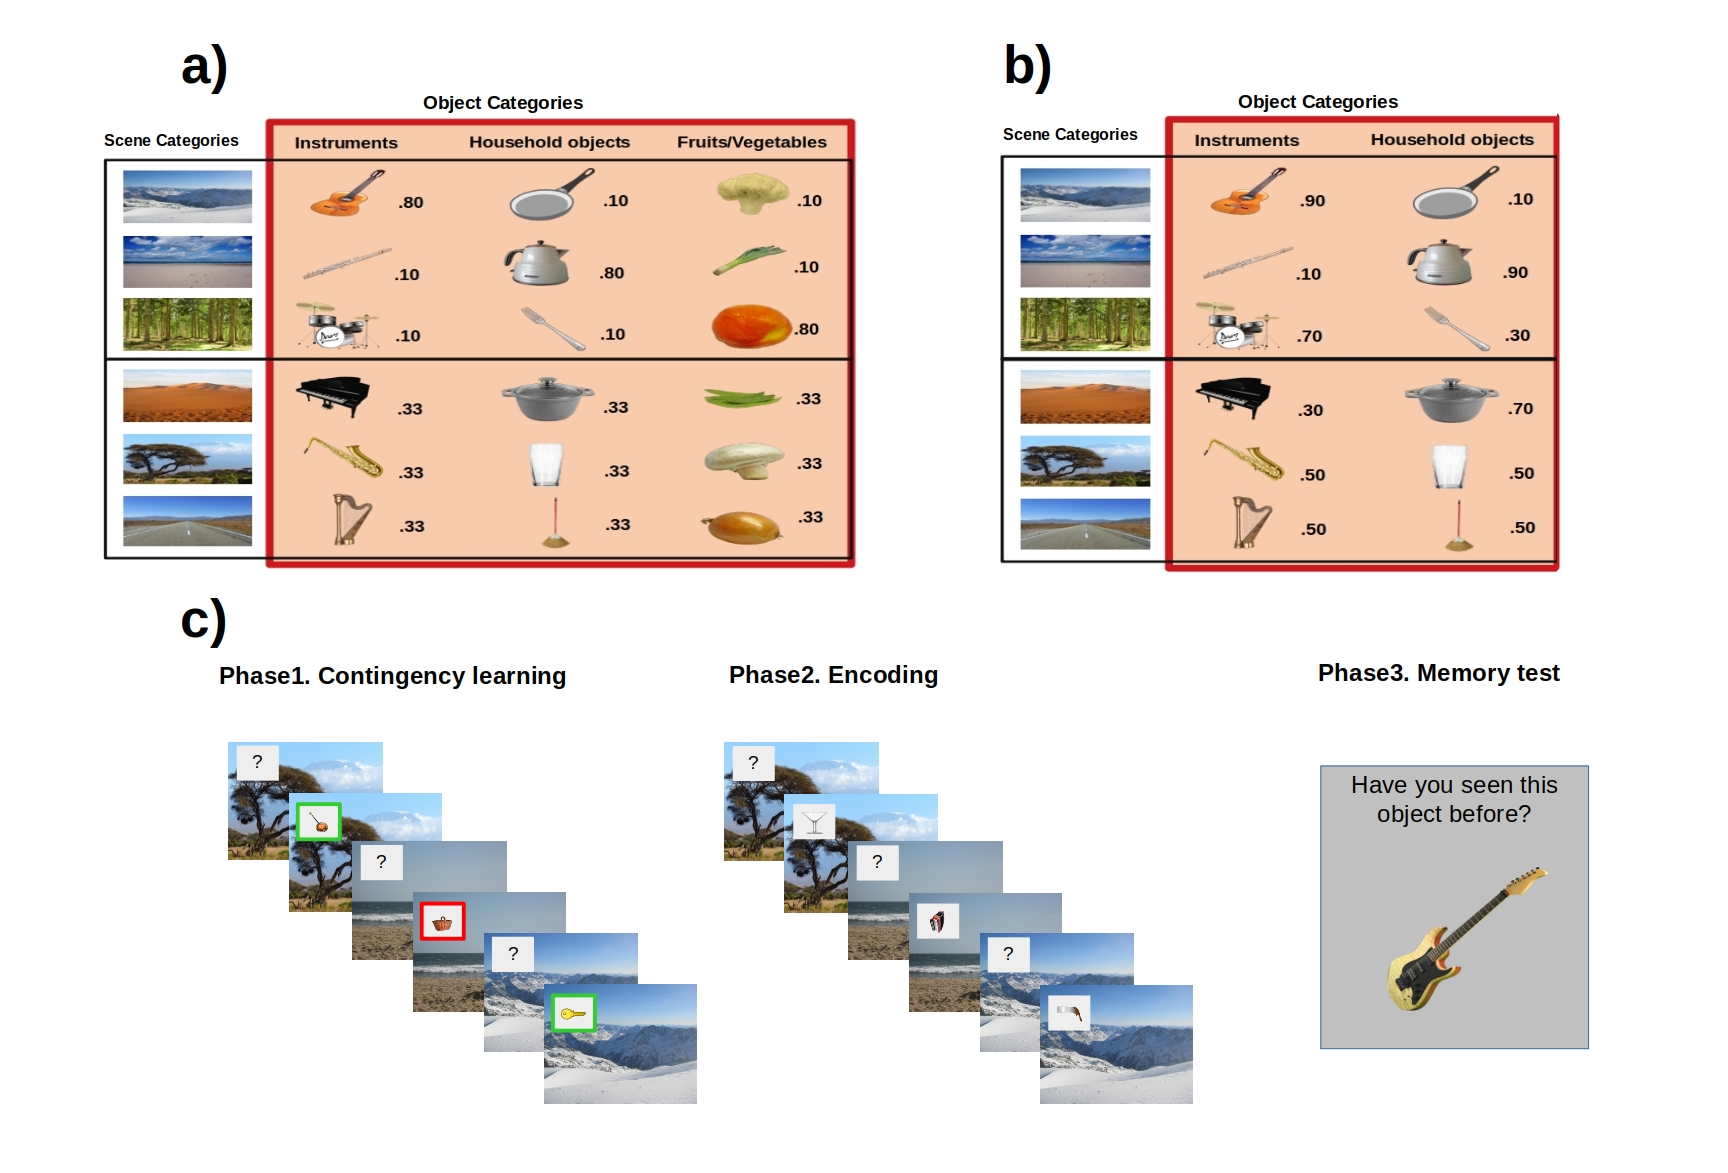
\includegraphics[width=1.5\textwidth]{figures/methods.All.jpg}}
\caption{\textbf{Illustration of the Methods.} 1. Illustration of the scene/object-category contingencies for the different prior conditions, for a) Experiment 1 and b) Experiment 2. Note that each object is a representative of its object category and that different items from each category where used for each cell shown here. 2. Illustration of the three phases of the study. }
\label{fig:Methods}
\end{figure}


In Experiment 1, participants were presented with six contexts. Each of the contexts was predictive of the object categories following specific contingencies (Figure \ref{fig:Methods}.1): half of contexts were used for the strong prior condition, in which one of the three objects categories was presented 80 \% of the times, and the remaining two object-categories 10 \% of the times; the other half of the contexts were used for the flat prior condition, in which all the three object categories were equally likely. In experiment 2, two instead of three object categories were used. The strong and the flat prior conditions were maintained, although with 90-10 and 50-50 contingencies, respectively, and a weak prior condition was introduced, with 70-30 contingencies. This manipulation allowed to sample more points along the PE continuum.

\subsection{Learning Performance}
Results of the learning and encoding phases task show that participants understood the task correctly and were able to learn to predict the object category that was more likely to be presented for each context, in both experiment 1 and experiment 2. Participants’ cumulative accuracy tended to approximate true probability for each context and experiment, as shown in Figure \ref{fig:participantsLer}.


\begin{figure}[ht!]
\centerline
{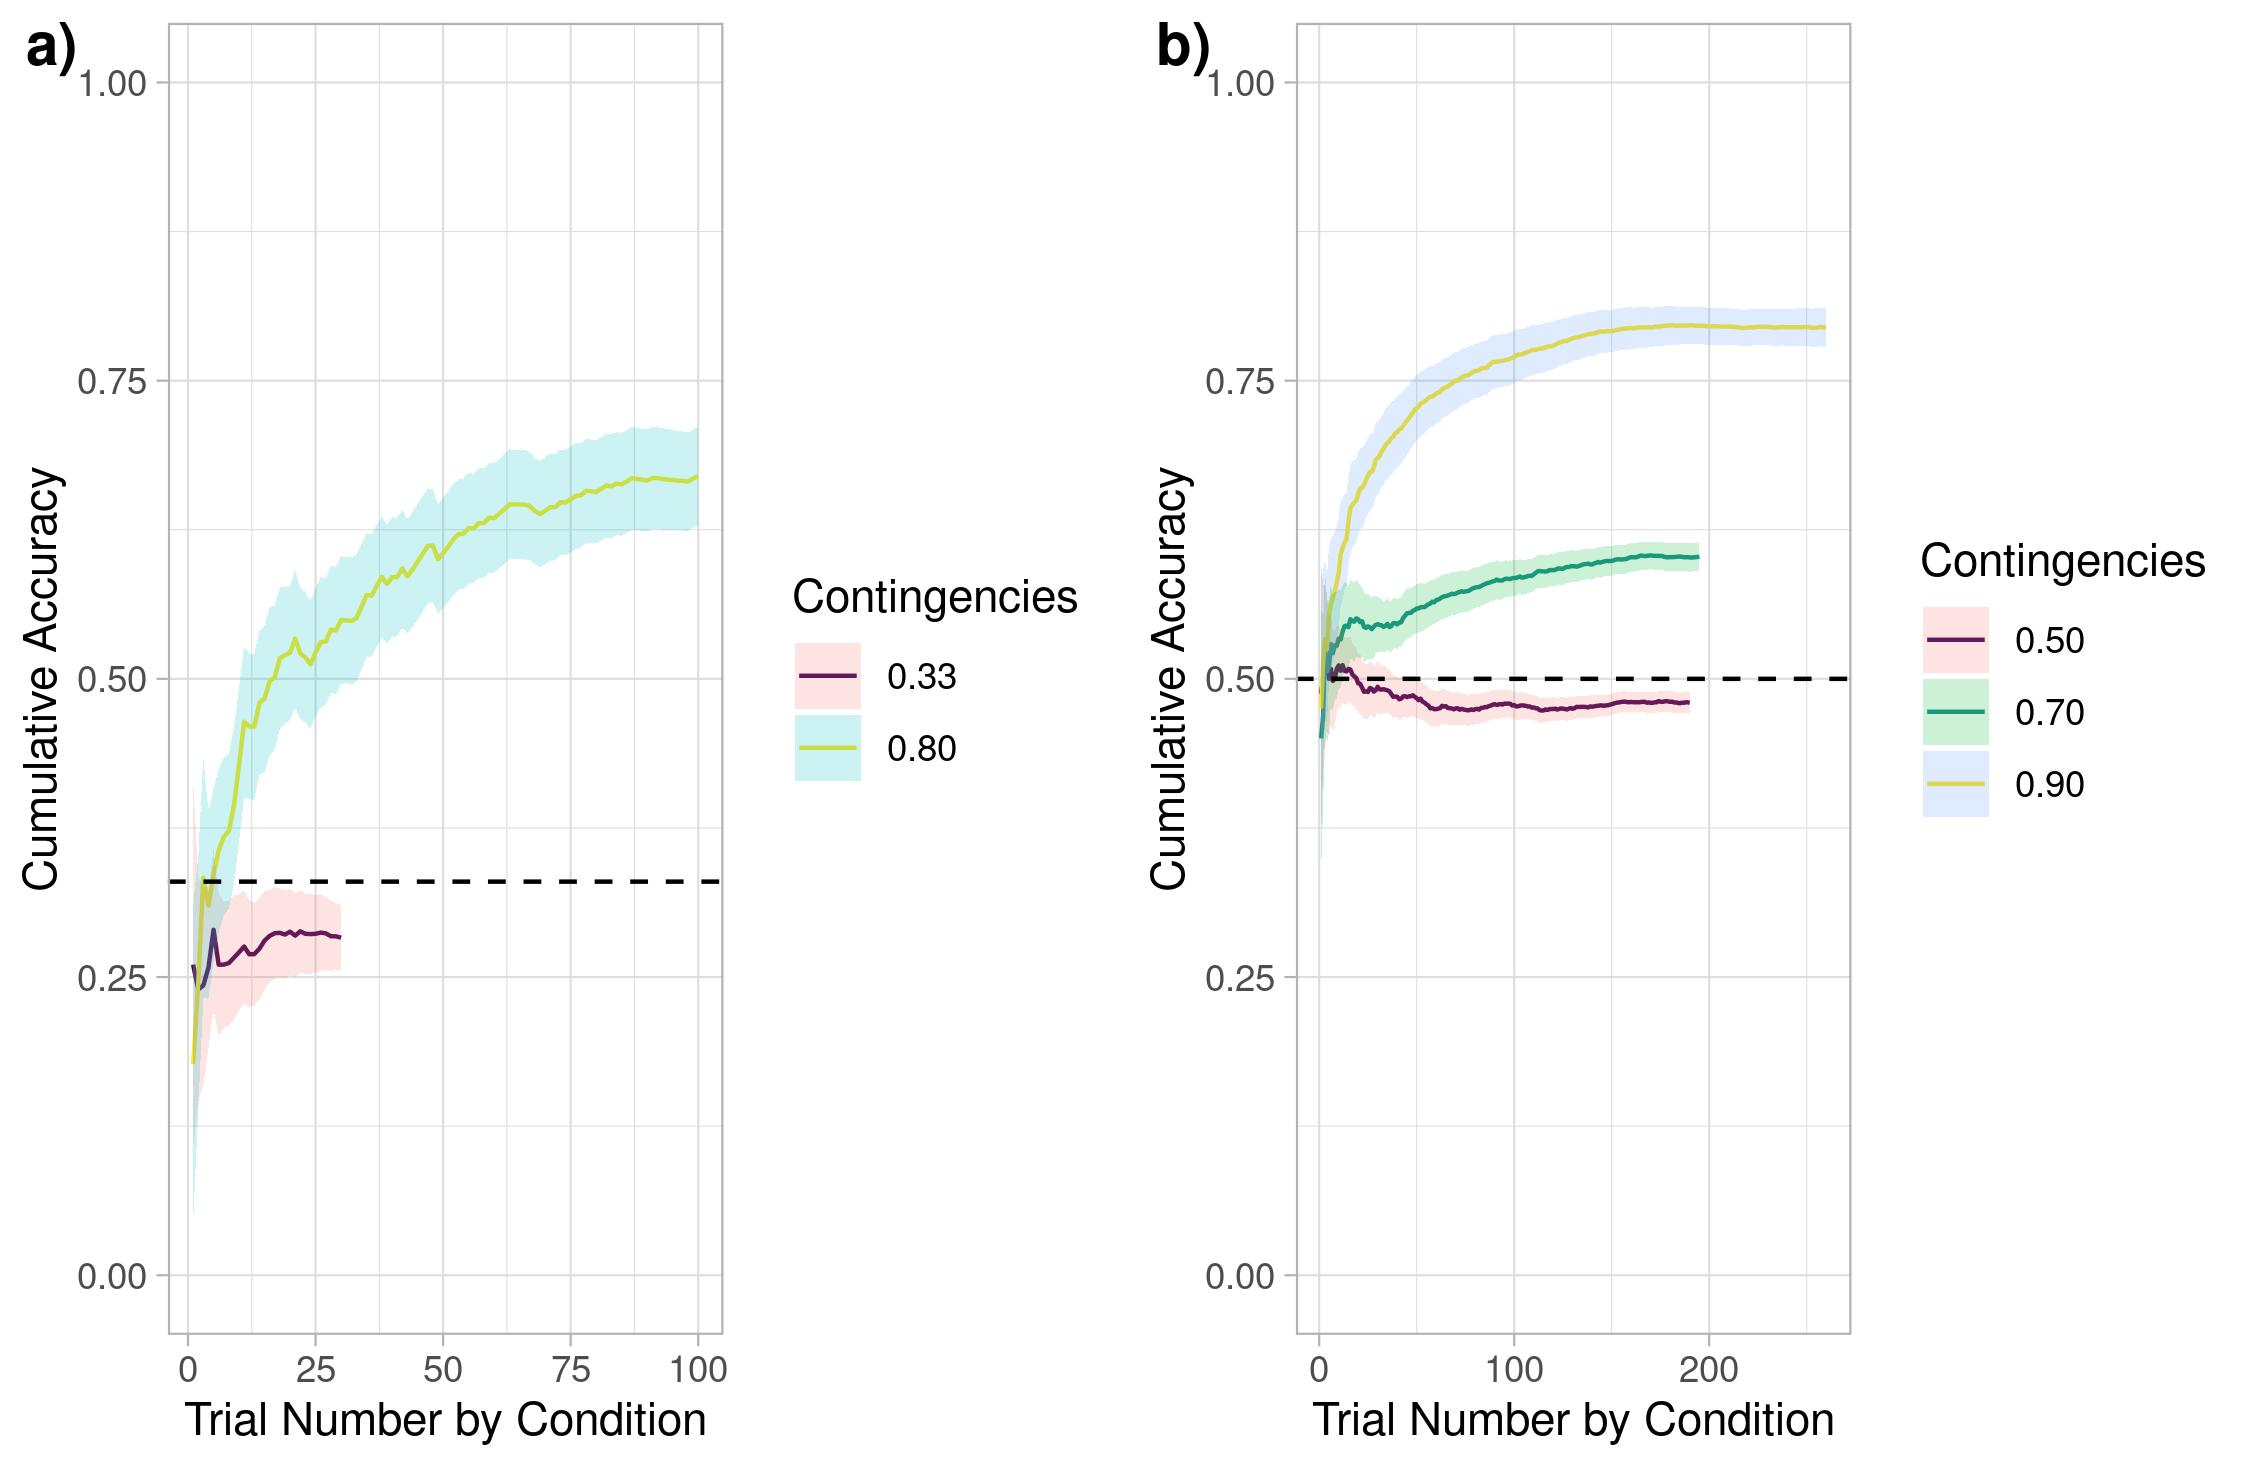
\includegraphics[width=1\textwidth]{figures/cumAccbySceneAll.jpg}}
\caption{\textbf{Participants' learning performance.} Participants' learning performance at the learning and encoding phase for a) experiment 1 and b) experiment 2. Trial number by condition (strong, weak, strong) is represented in the x axes, while cumulative accuracy is shown on the y axes. The different colours represent the scene conditions. Shadows represents standard error.}
\label{fig:participantsLer}
\end{figure}

\subsection{Computational Models}
In order to derive trial-level PE at encoding, different reinforcement learning models \citep{Sutton2018a} were fitted to behavioural data. The use of reinforcement learning models allowed to capture the process of establishing prior expectations by learning the object-category contingencies for the different contexts. In the reinforcement learning models, an agent is assume to learn values of context-category associations by adding the current expected value to a learning rate $\alpha$ multiplied by the PE. We fitted three different reinforcement learning models that made different assumptions on how participants learned the context/object-category associations (see Methods): An instructive model with a decreasing learning rate (dLRI), which updates the expected values on each trial through the observation of the outcomes, regardless of the choices made; An instructive model where participants were allowed to have their own learning rate $\alpha$ (fLRI), modelled as a free parameter; An evaluative model with a free learning rate (fLRE), where the expected values were updated through the outcome received on every trial. \par
The dLRI considers how the expected values should be updated optimally, since it is derived from a Bayesian formulation of the task (see Methods and Supplemental Material). In this optimal Bayesian formulation of learning during the task, the prediction error is assumed to have its maximal influence on learning in the early trials, to decrease immediately after as a function of the inverse of the number of the trials. In this model, the only parameter that was estimated was the 'inverse temperature' $\beta$, which regulates the stochasticity/determinism trade-off in selecting the action depending on the expected values: High values of $\beta$ represent more probable preference of the higher context/object-category associations, while lower values also consider low-strength associations, producing more noisy choices.
In addition to the $\beta$ parameter, and in contrast with the fixed decreasing learning rate of dLRI, the models fLRI and fLRE estimate a learning rate $\alpha$, a value between 0 and 1 that determines the influence of a current prediction error on the expected values. The learning rate represents the extent to which evidence from the current trial is used to update the expectations: Higher learning rate weights more the present evidence and the extend to which it deviates from the value estimates, while lower learning rate weights more the estimated values, and thus the past trials. \citep{Sutton2018a}.  \par
Prior to fitting the models to participants' data, we ensured that the models could distinguish among different parameters' value and also generate qualitatively different data (see 'Parameter Recovery' and 'Model Recovery' in Methods and Supplemental Material). Then, the three models were fit to participant's data, and the parameters of best fit were estimated as the parameters that maximized the likelihood of participant's choices. 

\subsubsection{Model Comparison}
In addition to calculating log-likelihood, we calculated the Bayesian information criterion (BIC) for each model and for each subject, by multiplying the maximum likelihood (i.e. the likelihood for the parameters of best fit) by the number of free parameters in the model. This approach penalizes models with more parameters. We then marked the number of participants for which each model was the best fit, as well as the evidence for it, computed as the BIC difference between the best and the second best model. Results are shown in Figure \ref{fig:ModelComparison}. Table \ref{tab:ModelComp} show BIC values and the the number of participants for which a model was the best fit, as well as the number of people for which there was strong evidence, for both Experiment 1 and Experiment 2. 


\begin{figure}[ht!]
\centerline
{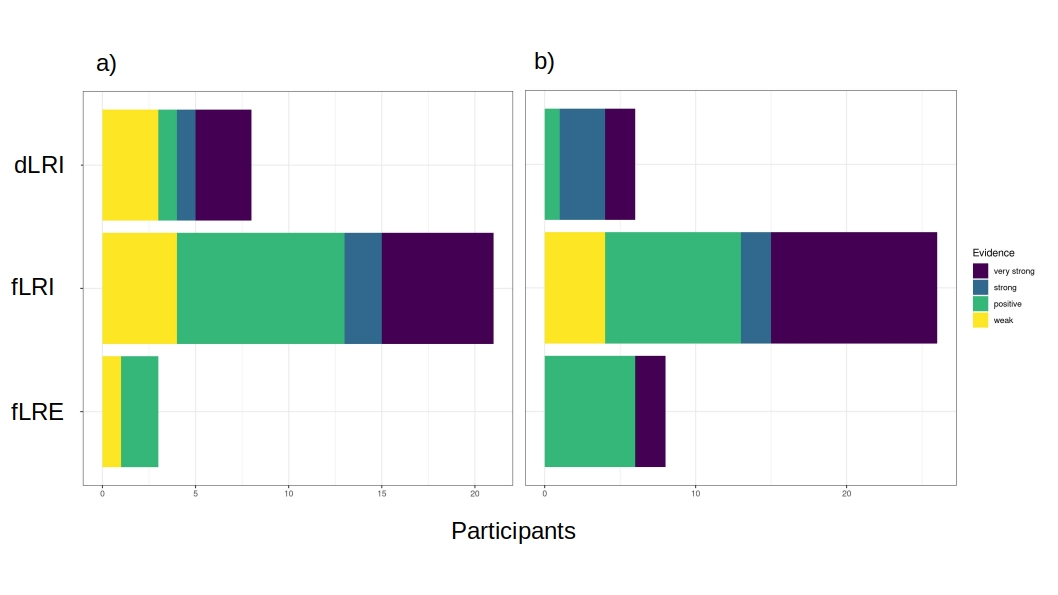
\includegraphics[width=1\textwidth]{figures/ModelComparisonAll.jpg}}
\caption{\textbf{Model Comparison.} Results of model comparison for a) experiment 1 and b) experiment 2. Evidence for the best model for each participants is shown.}
\label{fig:ModelComparison}
\end{figure}

\begin{table} 
    \centering 
    \caption{\label{tab:ModelComp}Model Comparison. BIC values and standard errors for each model for Experiment 1 and experiment 2. \textit{Best(N)} and \textit{Very strong(N)} refer to the number of participants for which the model was the best fit and for which there was very strong evidence, respectively   }
    \scalebox{1}{
    \begin{tabular}{l l l l}

     \hline

   Model/Experiment & BIC (\textit{se}) & Best(N) & Very Strong (N) \\
     \hline
    \textbf{Experiment 1} \\ 

  dLRI & 289.3(3.1) & 3 & 0 \\
  fLRI & 266.4(1.5) & 21 & 6 \\
  fLRE & 271.4(2.4) & 8 & 3 \\

         \textbf{Experiment 2} \\
  dLRI & 801.2(4.9) & 8 & 2 \\
  fLRI & 783.1(2.3) & 26 & 11 \\
  fLRE & 774.3(3.2) & 6 & 2 \\
     \hline

    \end{tabular}
}
    \end{table}

Model comparison established that the instructive model with the free learning rate (fLRI) explained participants behaviour better than the other models. In fact, the overall BIC was smaller (indicating better fit), and the number of participants for which it was the best model were 21 over 32 for experiment 1, and 26 over 40 for experiment 2. In addition, there was very strong evidence for it being the best model for 6 participants in experiment 1 and 11 participants in experiment 2. Therefore, the best fitting model was the model that considers instructive feedback and estimates a specific learning rates for each participant.  

\subsubsection{Model Validation}
We then analysed the ability of the model to generate performance which was qualitatively similar to participants' actual behaviour. For each actual participant, we simulated data on the learning and encoding tasks using the best fitting model (fLRI) and its estimation of best fitting parameters. The model simulations included the actual task structure. In order to evaluate model's simulations, we calculated cumulative accuracy for the data generated by the model and qualitatively compared it to participants' actual cumulative accuracy. Figure \ref{fig:simvsemp_Exp1} and Figure \ref{fig:simvsemp_Exp2} show that the simulated models capture participants' behaviour.


\begin{figure}[ht!]
\centerline
{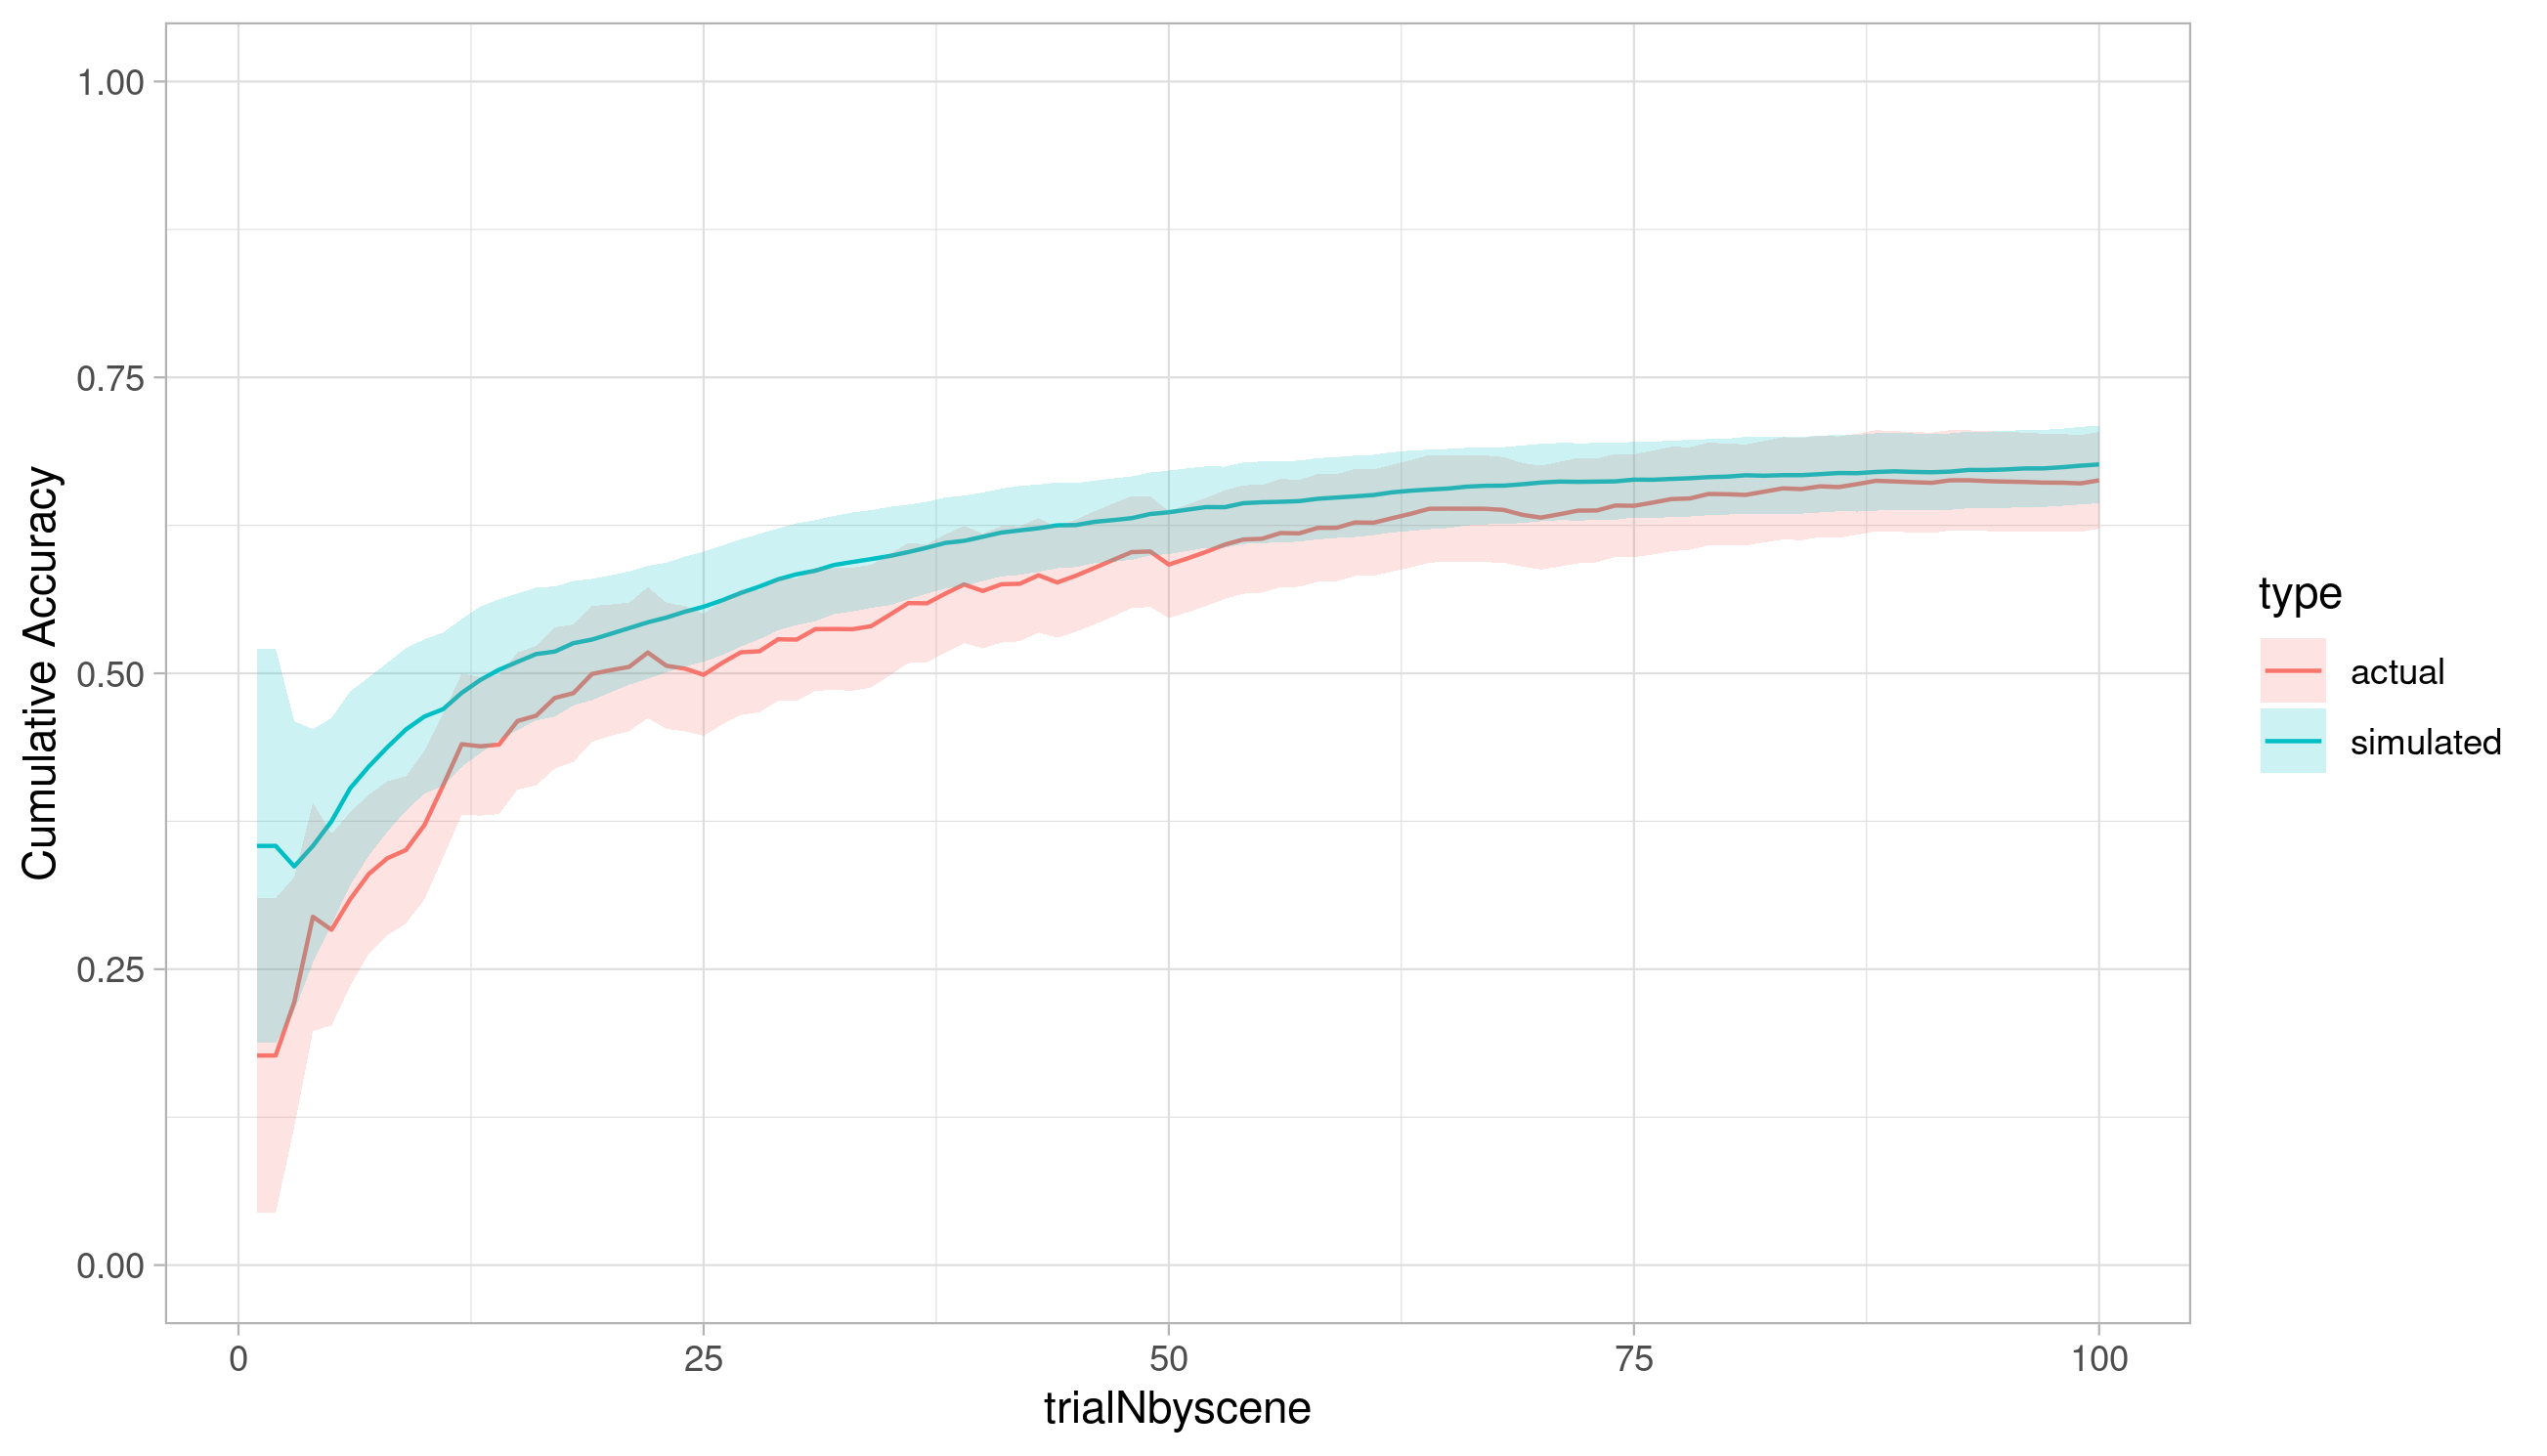
\includegraphics[width=1\textwidth]{figures/SimulatedVsActual.exp=exp1.mod=fLR_Instr.png}}
\caption{\textbf{Simulated vs Empirical Data - Experiment 1.} Simulated data (red line) and actual data (green line) overlapped, for experiment 1.}
\label{fig:simvsemp_Exp1}
\end{figure}

\begin{figure}[ht!]
\centerline
{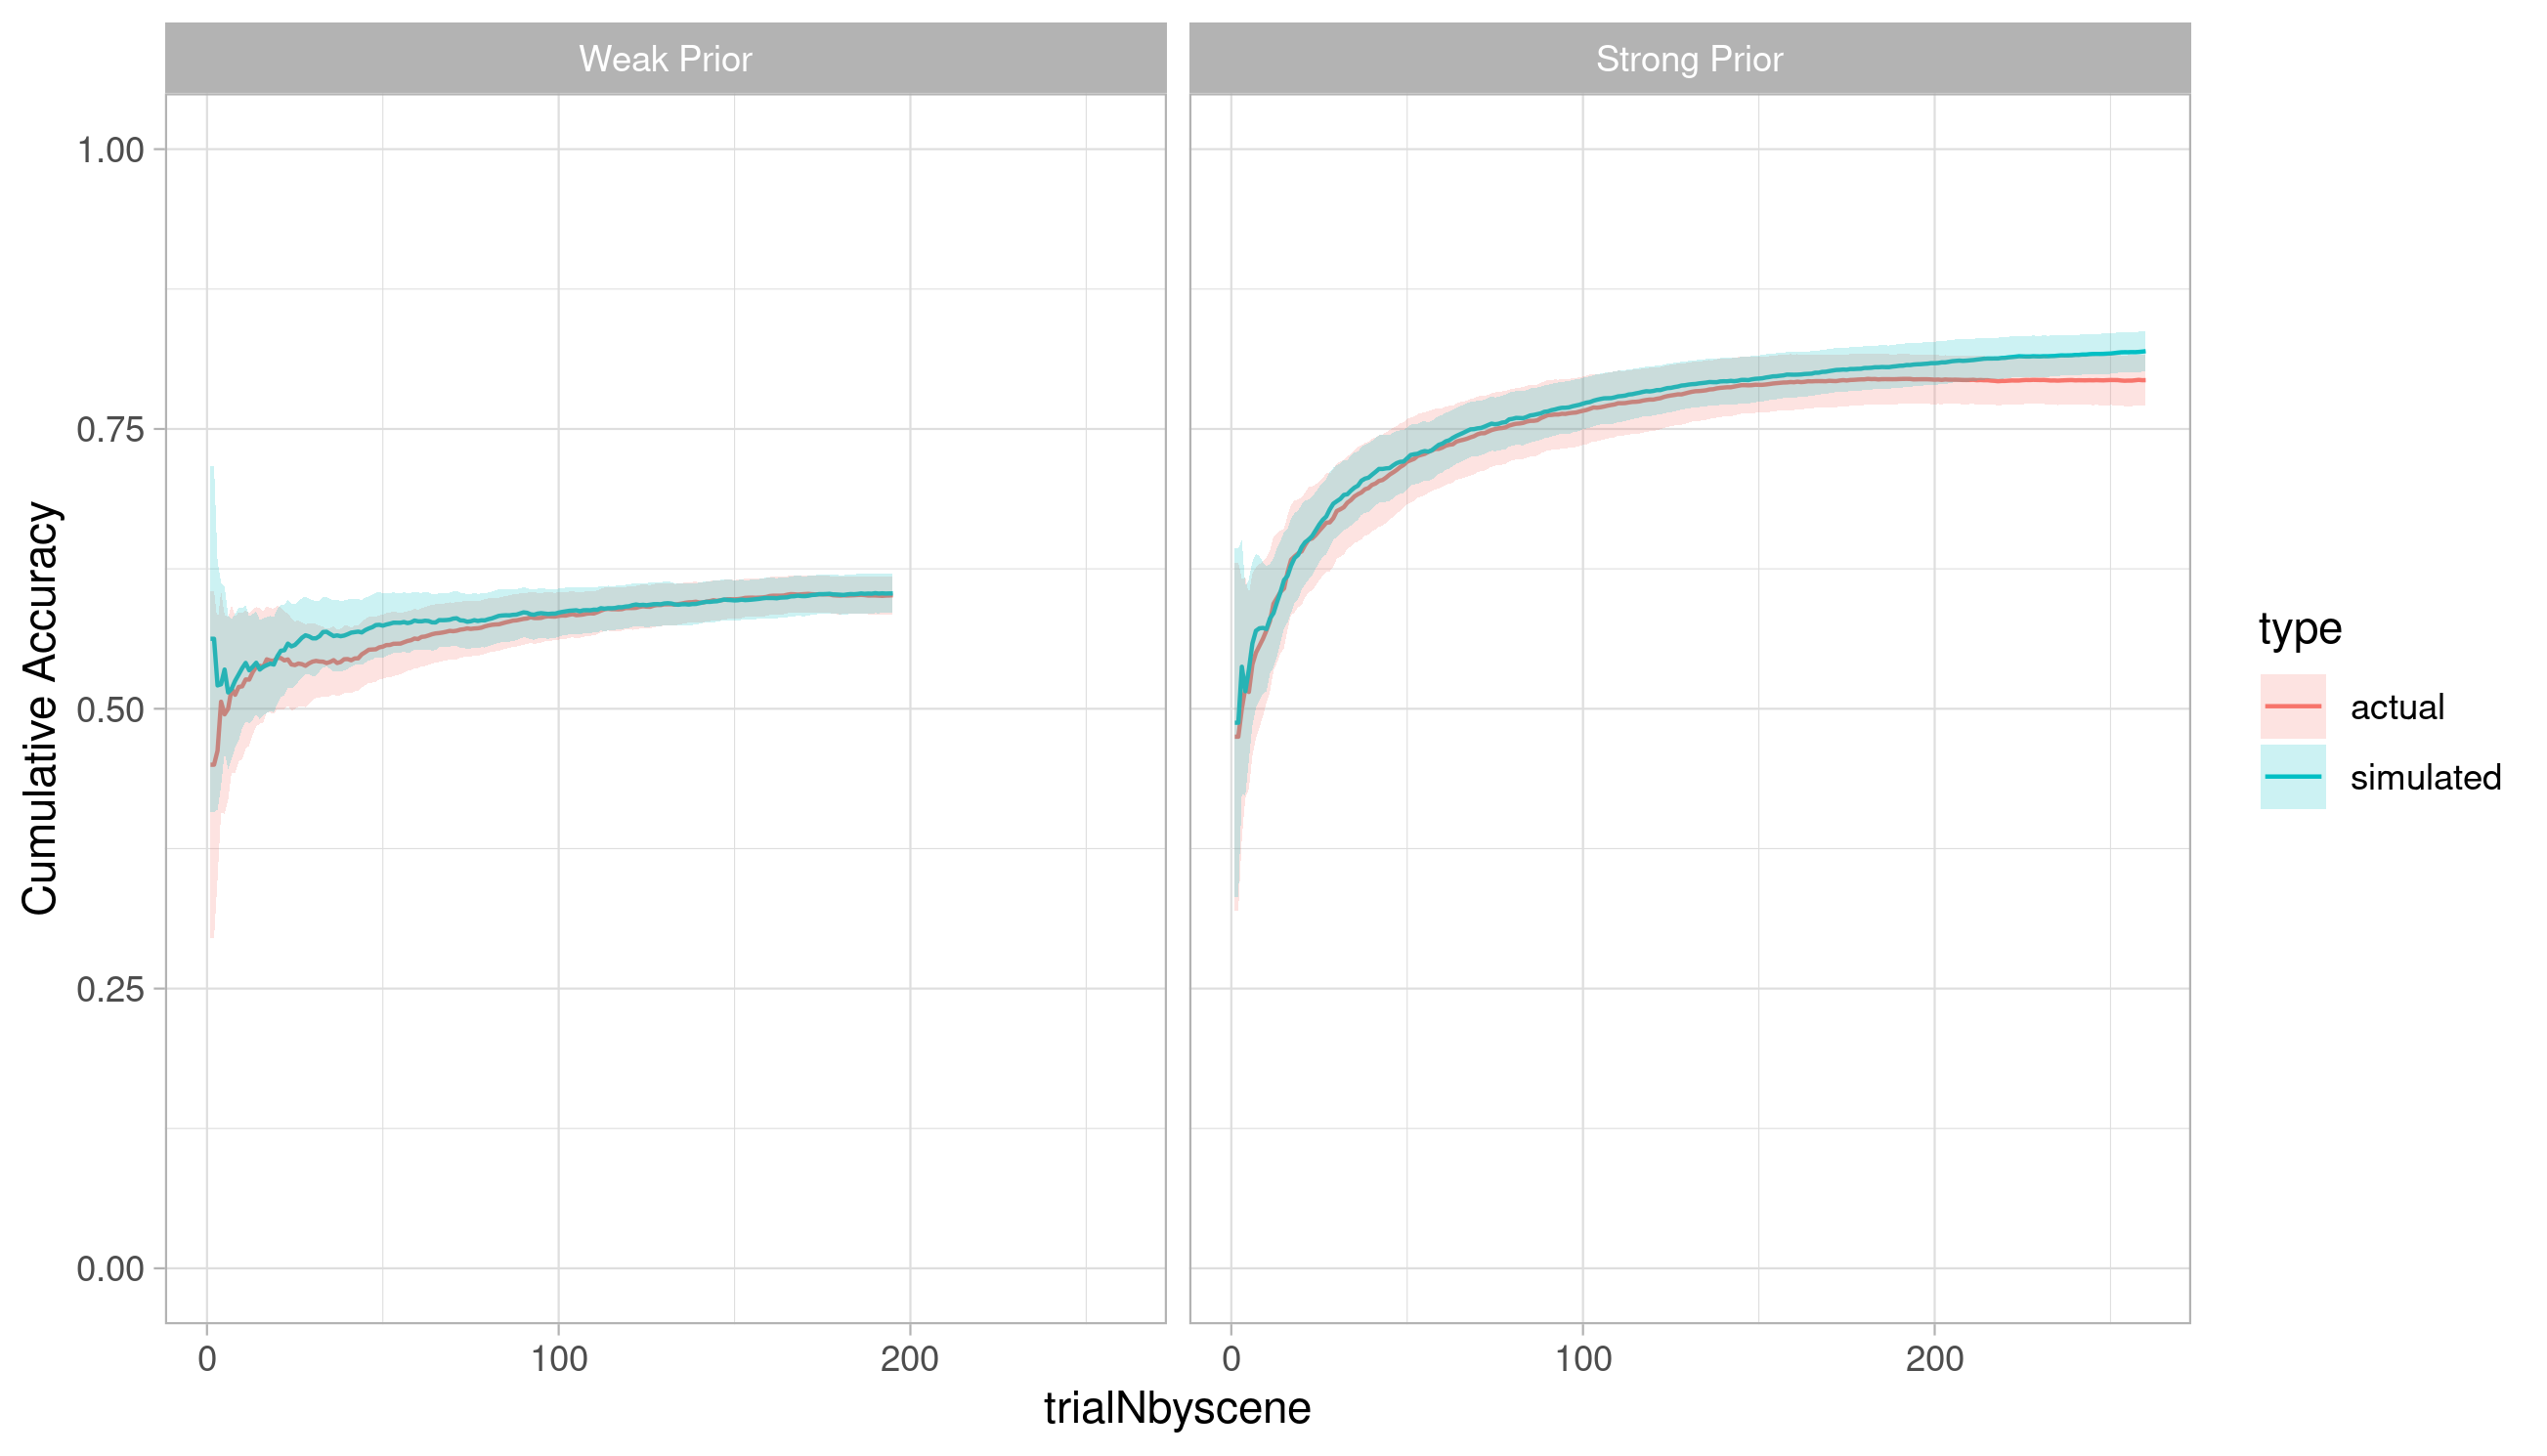
\includegraphics[width=1.5\textwidth]{figures/SimulatedVsActual.exp=exp2.mod=fLR_Instr.png}}
\caption{\textbf{Simulated vs Empirical Data - Experiment 2.} Simulated data (red line) and actual data (green line) overlapped, for experiment 2, for weak priors condition and strong prior condition. }
\label{fig:simvsemp_Exp12}
\end{figure}

In addition, we compared cumulative accuracy for simulated and empirical data at different values of learning rate $\alpha$. For simulated and empirical data, quartiles for $\alpha$ were calculated (zeroth, first, second, third, and fourth quartile), and cumulative accuracy was aggregated for the data points between one quartile and the previous one. Cumulative accuracy for the four bins created is shown in Figure \label{fig:binAll}, as a function of order of the trials (late vs early), type of data (empirical vs simulated), and experiment (first vs second experiment). For both actual and simulated data, a higher learning rate was more beneficial than a lower one for early trials, while on late trials higher learning rates are detrimental for the learning task. These effects seem not to vary substantially as a function of the experiment. 

\begin{figure}[ht!]
\centerline
{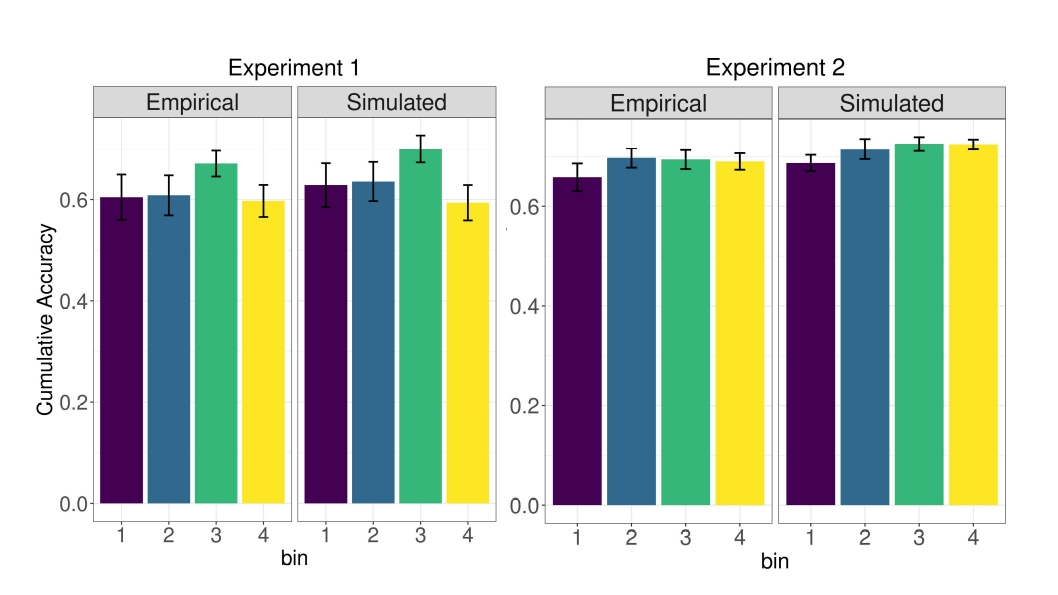
\includegraphics[width=1.5\textwidth]{figures/bin.plot.all.jpg}}
\caption{\textbf{Cumulative Accuracy for Simulated and Empirical by Learning Rate.} Figures show the cumulative accuracy at the leaning task for early vs late trials, at different learning rate levels, for a) experiment 1 and b) esperiment two. Cumulative accuracy was binned  }
\label{fig:binAll}
\end{figure}

\subsection{Recognition Memory Results}
To evaluate overall memory performance for each participant, a d' score was calculated from the hits (responding "old" to old items) and false alarms (responding "old" to new items), an index which indicates participants' ability to discriminate between old and new items. In order to exclude participants who did not perform the task above chance levels, we created a null distribution by generating 5000 random permutations of the trial labels. We then excluded participants whose performance was below the 95 \% percentile of the distribution. Five participants from experiment 1 and five from experiment 2 with overall d' score below the obtained threshold were excluded from further analyses. After the exclusion, the final d' was d' = 0.93,  \textit{t}(26) = 13.7, \textit{p} < .001 for experiment 1, and d’ = 0.90,  \textit{t}(34) = 16.8, \textit{p} < .001 for experiment 2, indicating that participants were overall able to discriminate previously presented old items from new distractors. 

\subsection{Memory as a function of model-derived PE}
The fLRI model was fit to participant data with the estimated best fit parameter in order to derive trial-level PE during the encoding phase. PE was calculated as the difference between whether or not an object category was presented (1 or 0, respectively) and its current estimated value (the strength of the expectation that an object category would be presented at a given scene). Higher PE levels were generated when a category presented was not expected, as reflected by its corresponding expected value being close to zero. By contrast, lower PE was generated by trials in which the category presented was characterized by a high expected value. Distribution of PE by prior conditions for experiment 1 and 2 is shown in Figure \ref{fig:PE_distr}. 

\begin{figure}[ht!]
\centerline
{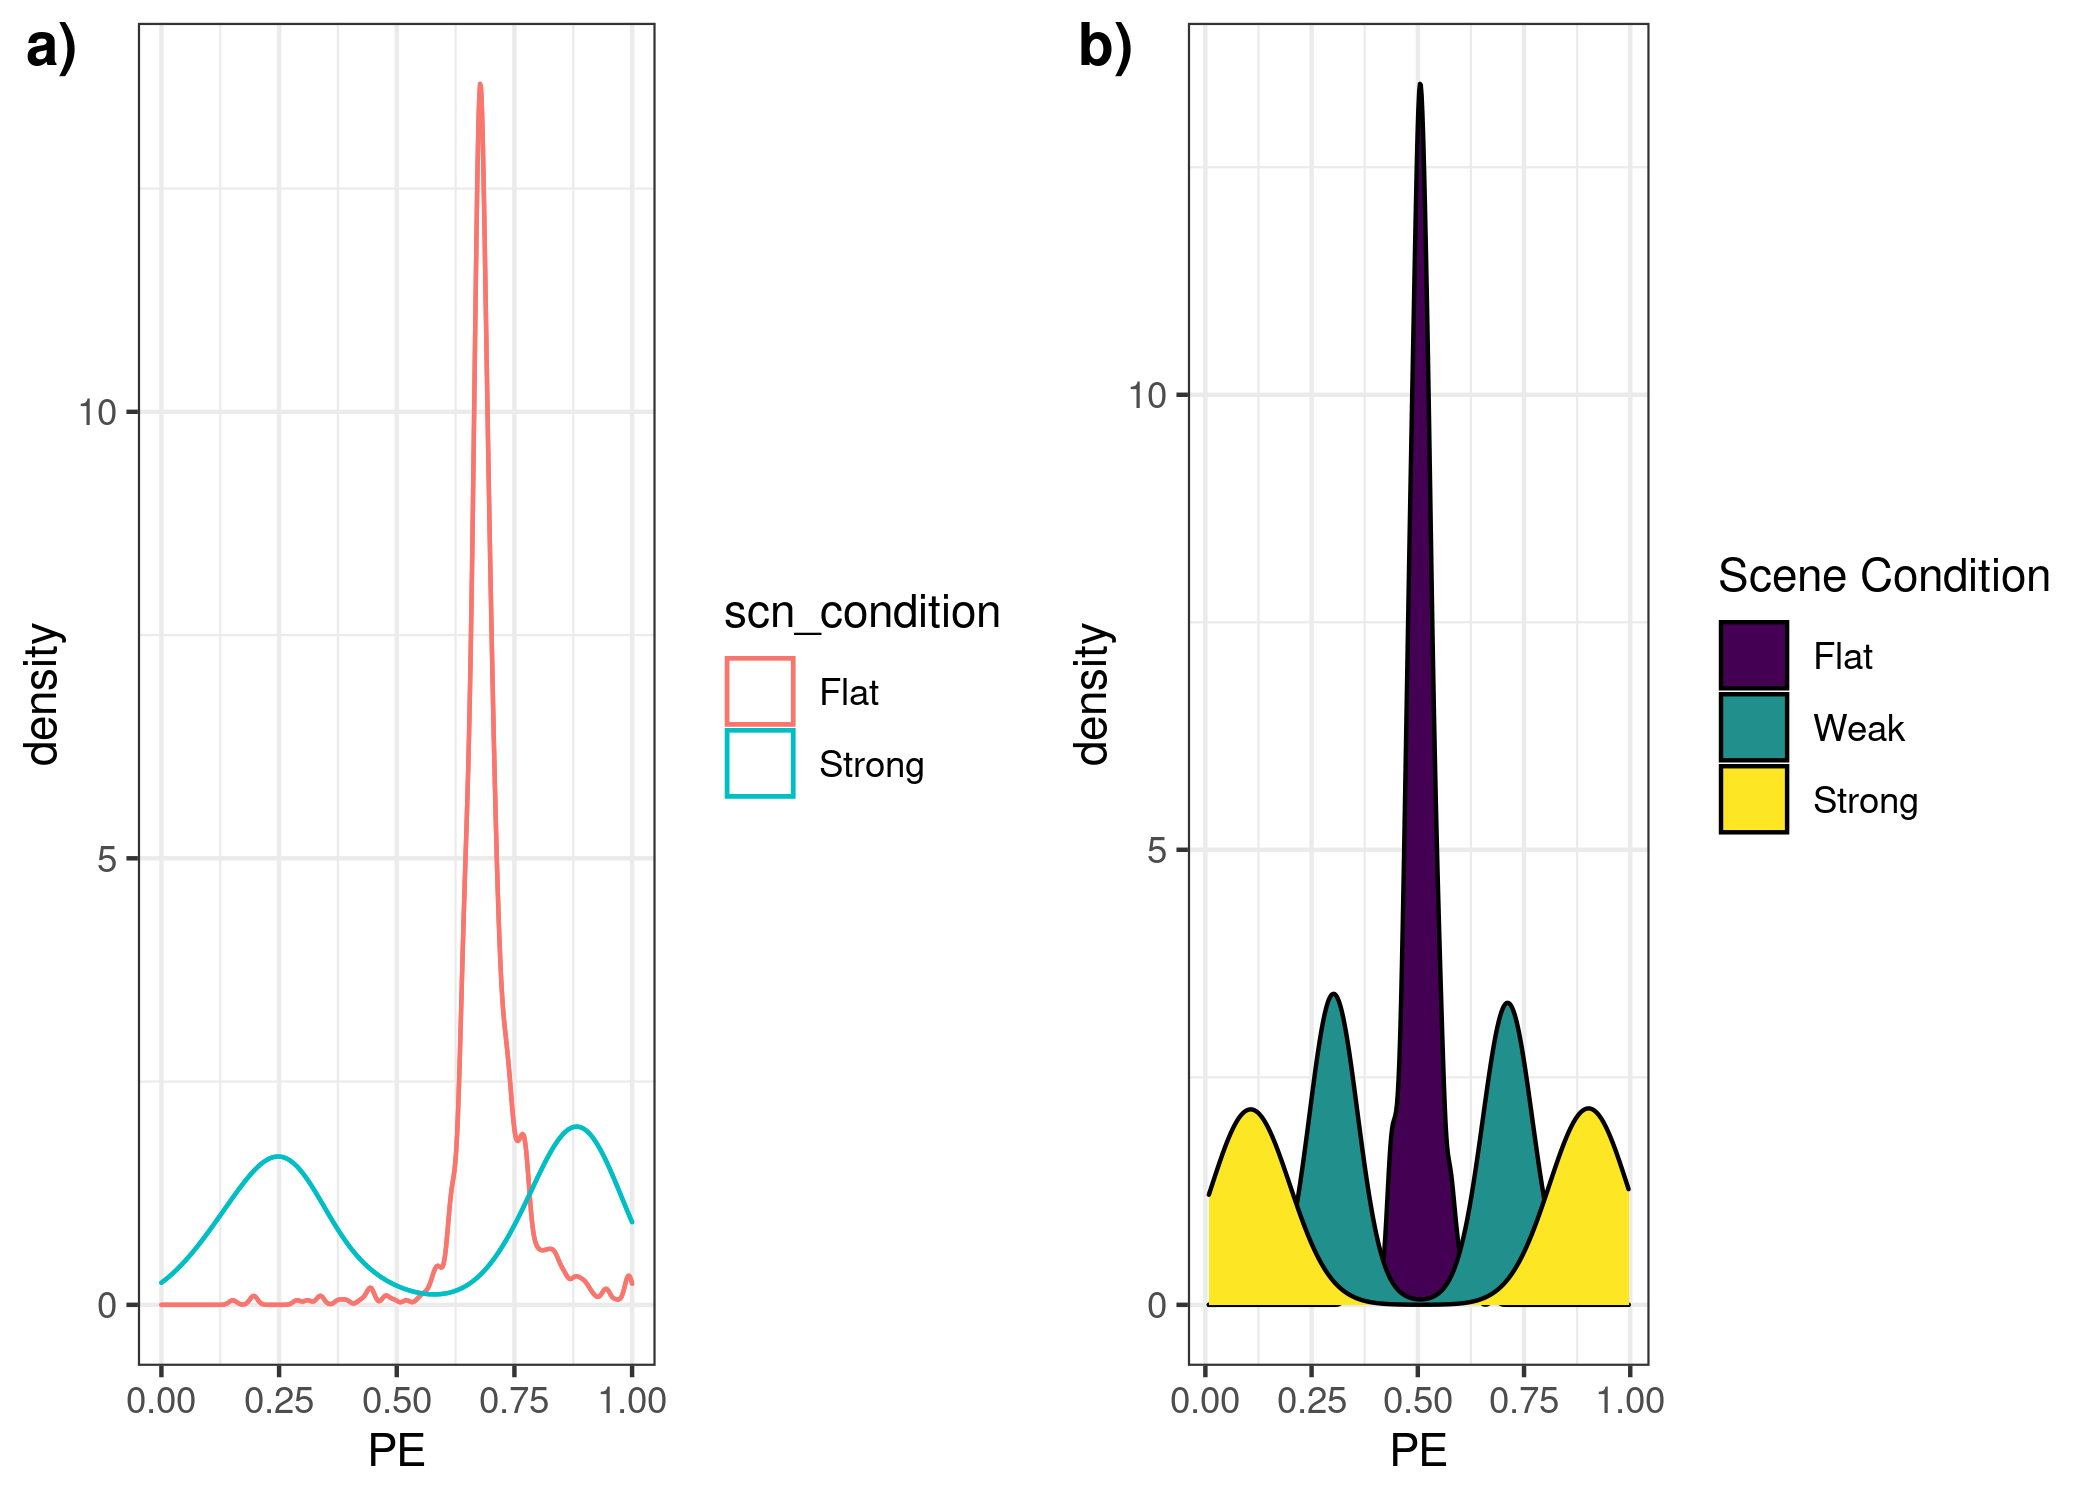
\includegraphics[width=1.5\textwidth]{figures/PEdistr_fLR_instr.All.png}}
\caption{\textbf{Distribution of PE by Scene Condition and Experiment.} Figures show the density plots of model-derived PE for the different scene conditions, in a) experiment 1 and b) experiment 2.  }
\label{fig:PE_distr}
\end{figure}

The plots shows that PE was distributed differently as a function of the scene condition. The bimodal distribution in the weak and the strong prior conditions represents the congruent and incongruent items: Items that matched expectations generated distributions of PE centered at lower values, while items that mismatched expectation generated PE distributions centered at higher values. For flat prior conditions, the distribution of PE was centered at one minus the probability that an object-category was presented, given that expectations are zero (1-0.33 for Experiment 1, 1-0.50 for Experiment 2). \par
We then tested whether model-derived PE was related to recognition memory. Plots of the observed values (see Figure \ref{fig:PE_mem}) showed a relationship between PE and memory modulated by prediction outcome. In order to statistically test for the significance of this relationship, we used a generalized linear-mixed model were participants were treated as random effects (see Methods). In the model, PE and prediction outcome, as well as their interactions, were added as fixed effects. In addition, random slopes for PE and prediction outcome, and their interaction, were also added to the model. Analysis revealed a significant interaction between PE and prediction outcome ( $\chi^2_{(1)}$ = 10.46, \textit{p} = .001, Experiment 1;  $\chi^2_{(1)}$ = 13.74, \textit{p} < .001, Experiment 2).


\begin{figure}
{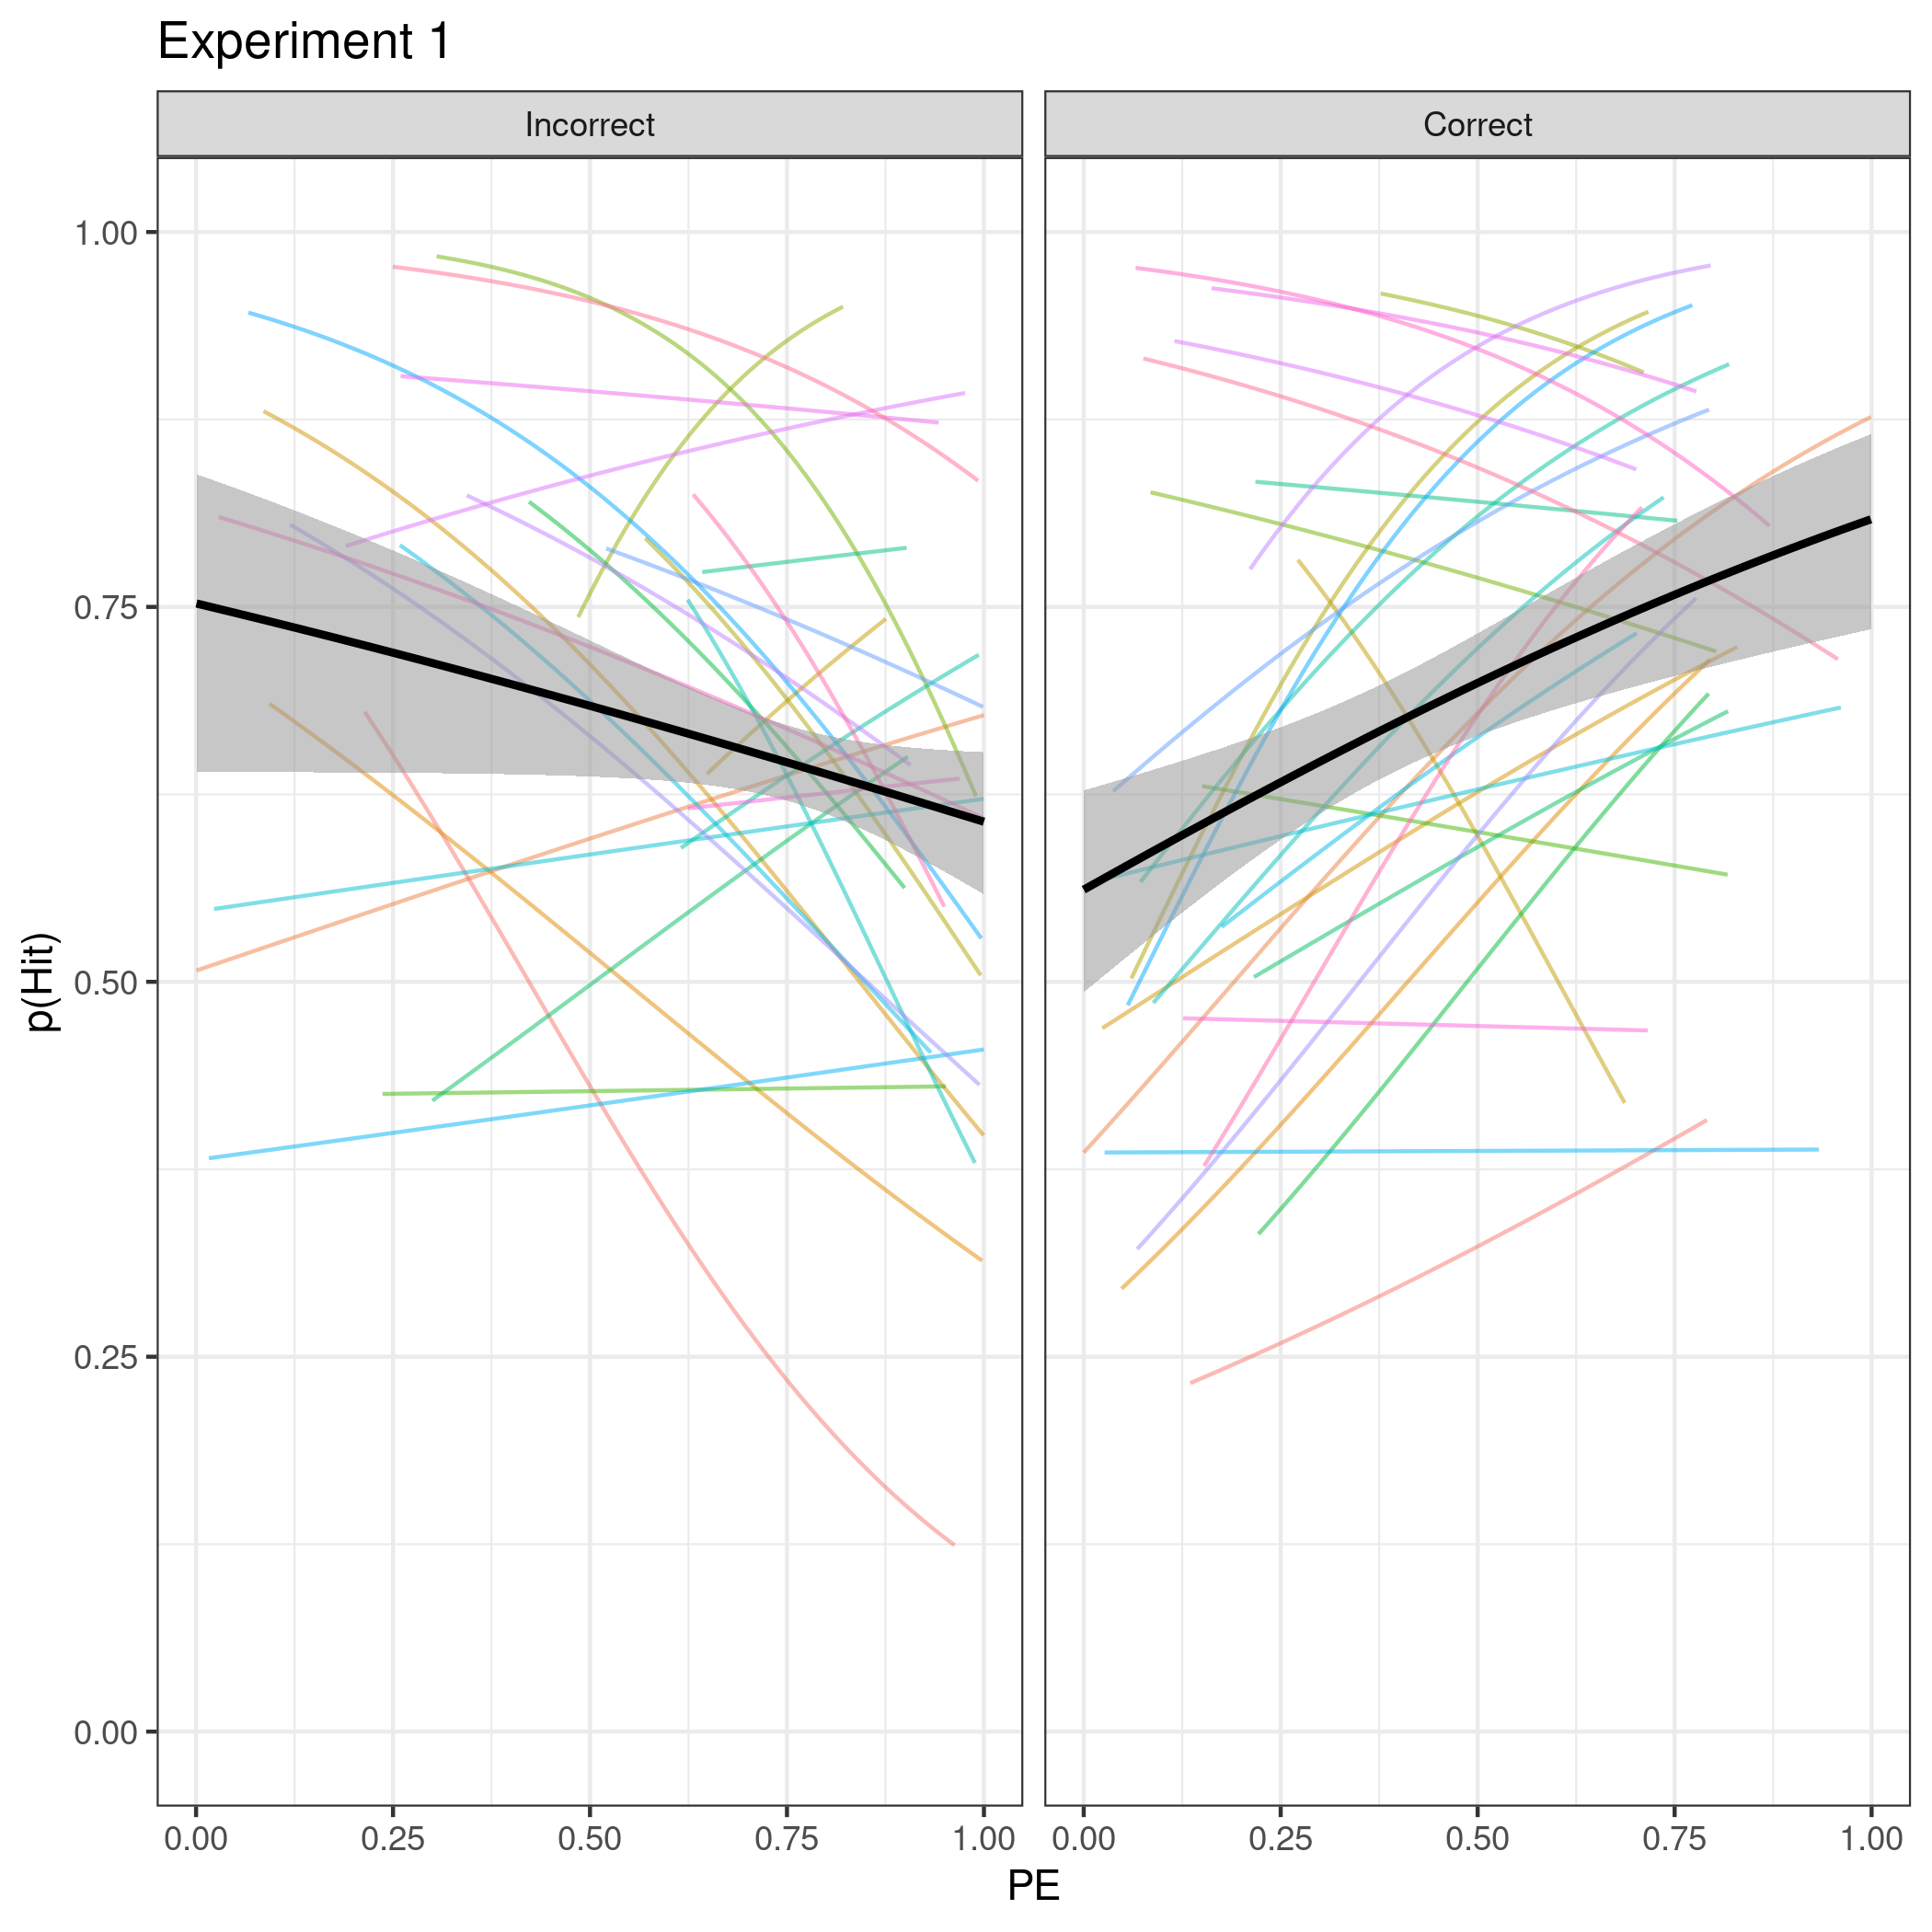
\includegraphics[width=0.75\textwidth]{figures/PE_mem_fLR_instr.exp1.png}}\hfill
{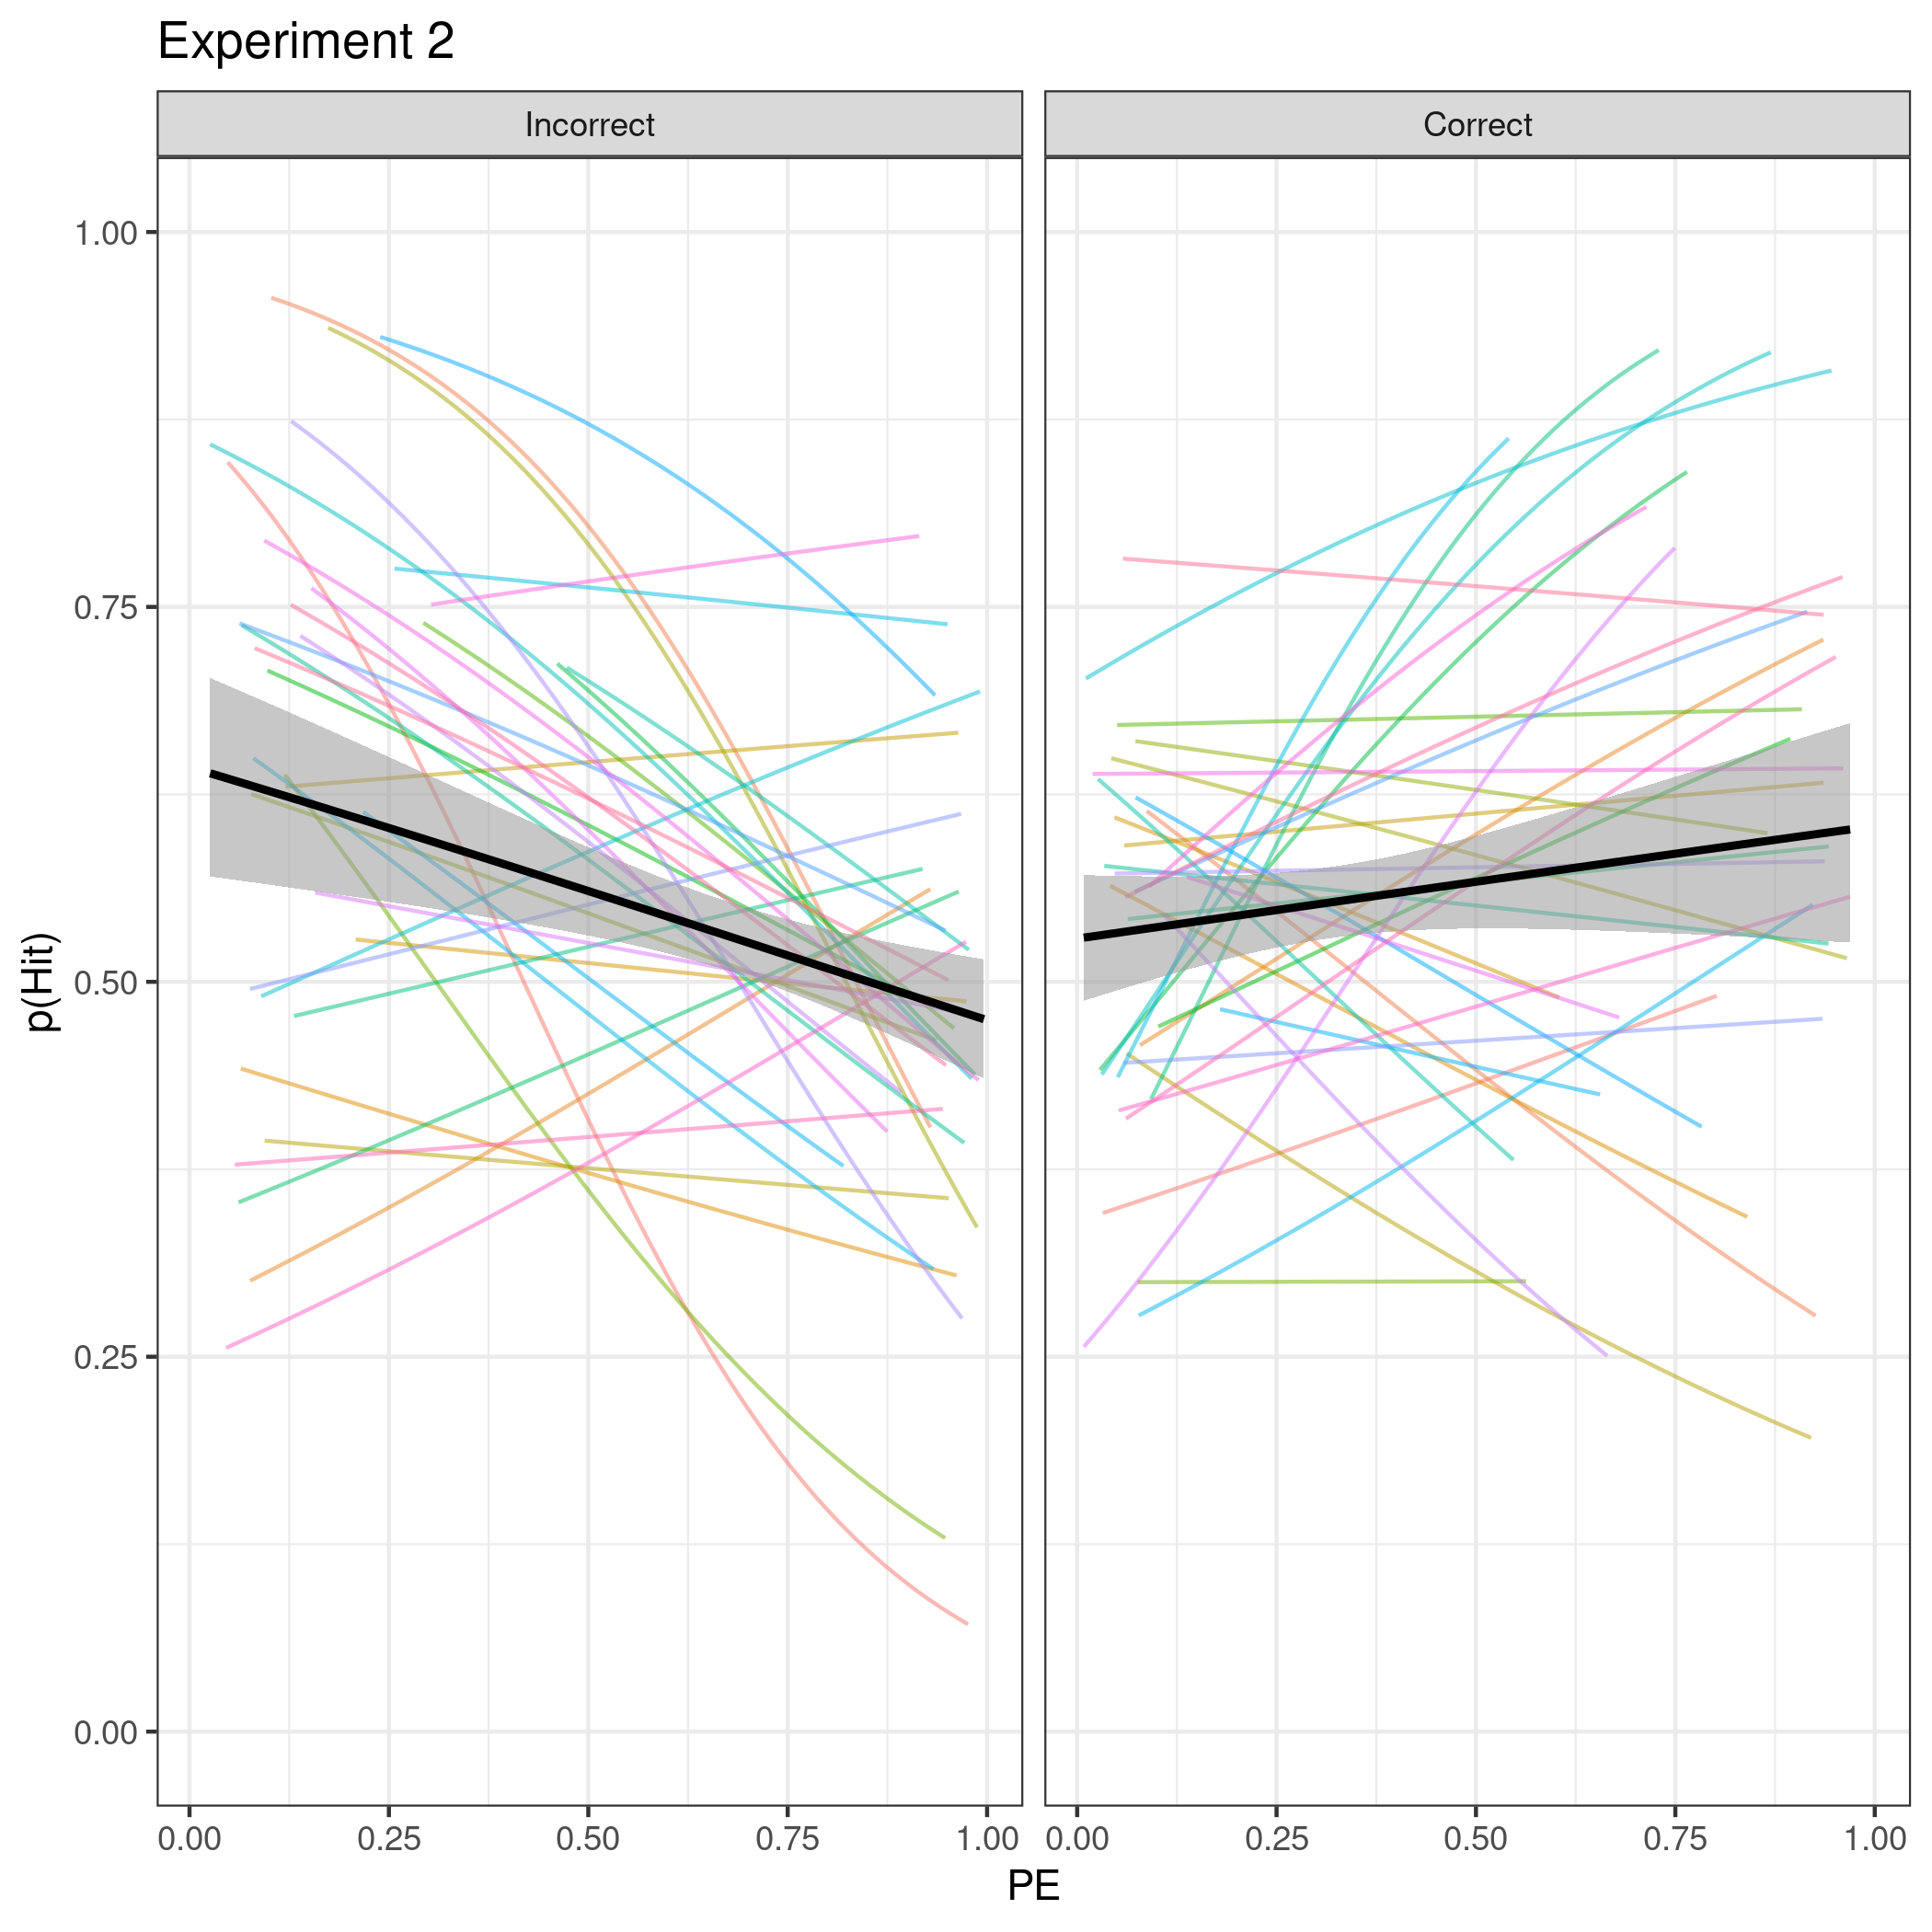
\includegraphics[width=0.75\textwidth]{figures/PE_mem_fLR_instr.exp2.png}}\
\caption{\textbf{PE and Memory as a function of Prediction Outcome.} Observed relationship between PE and hit rate as a function of prediction outcome, in experiment 1 and experiment 2. }
\label{fig:PE_mem}

\end{figure}


To break down the interactions, we analyzed the effect of PE on memory separately for correct and incorrect predictions. For Experiment 1, there was a positive linear relationship between PE and recognition memory when prediction outcome was correct, $\beta$ = 1.14, \textit{p} = .002, OR = 3.13, while a negative linear trend when prediction outcome was incorrect which did not reach significance, $\beta$ = - 0.83, \textit{p} = .071, OR = 2.29. For Experiment 2, a positive linear trend between PE and recognition memory when predictions were correct did not reach significance, $\beta$ = 0.39, \textit{p} = .111, OR = 1.45, while there was a significant negative relationship for incorrect predictions, $\beta$ = - 0.862, \textit{p} < .001, OR = 2.36. 

\paragraph{Analysis of Experiment 1 and Experiment 2 merged.}
As a next step, we merged data from both experiments and analyzed them in the same model to increase power. In order to compare memory at different levels of the model-derived PE, we calculated the quartiles for PE for each participant, separately for trials with correct and incorrect prediction outcome. We then binned the hit rate by aggregating it between the quartiles, to create four bins which eventually were used as the explanatory variable in our analysis. A graph with the distribution of PE by binned data is shown in Figure \ref{fig:PEbin_distr}.

\begin{figure}[ht!]
{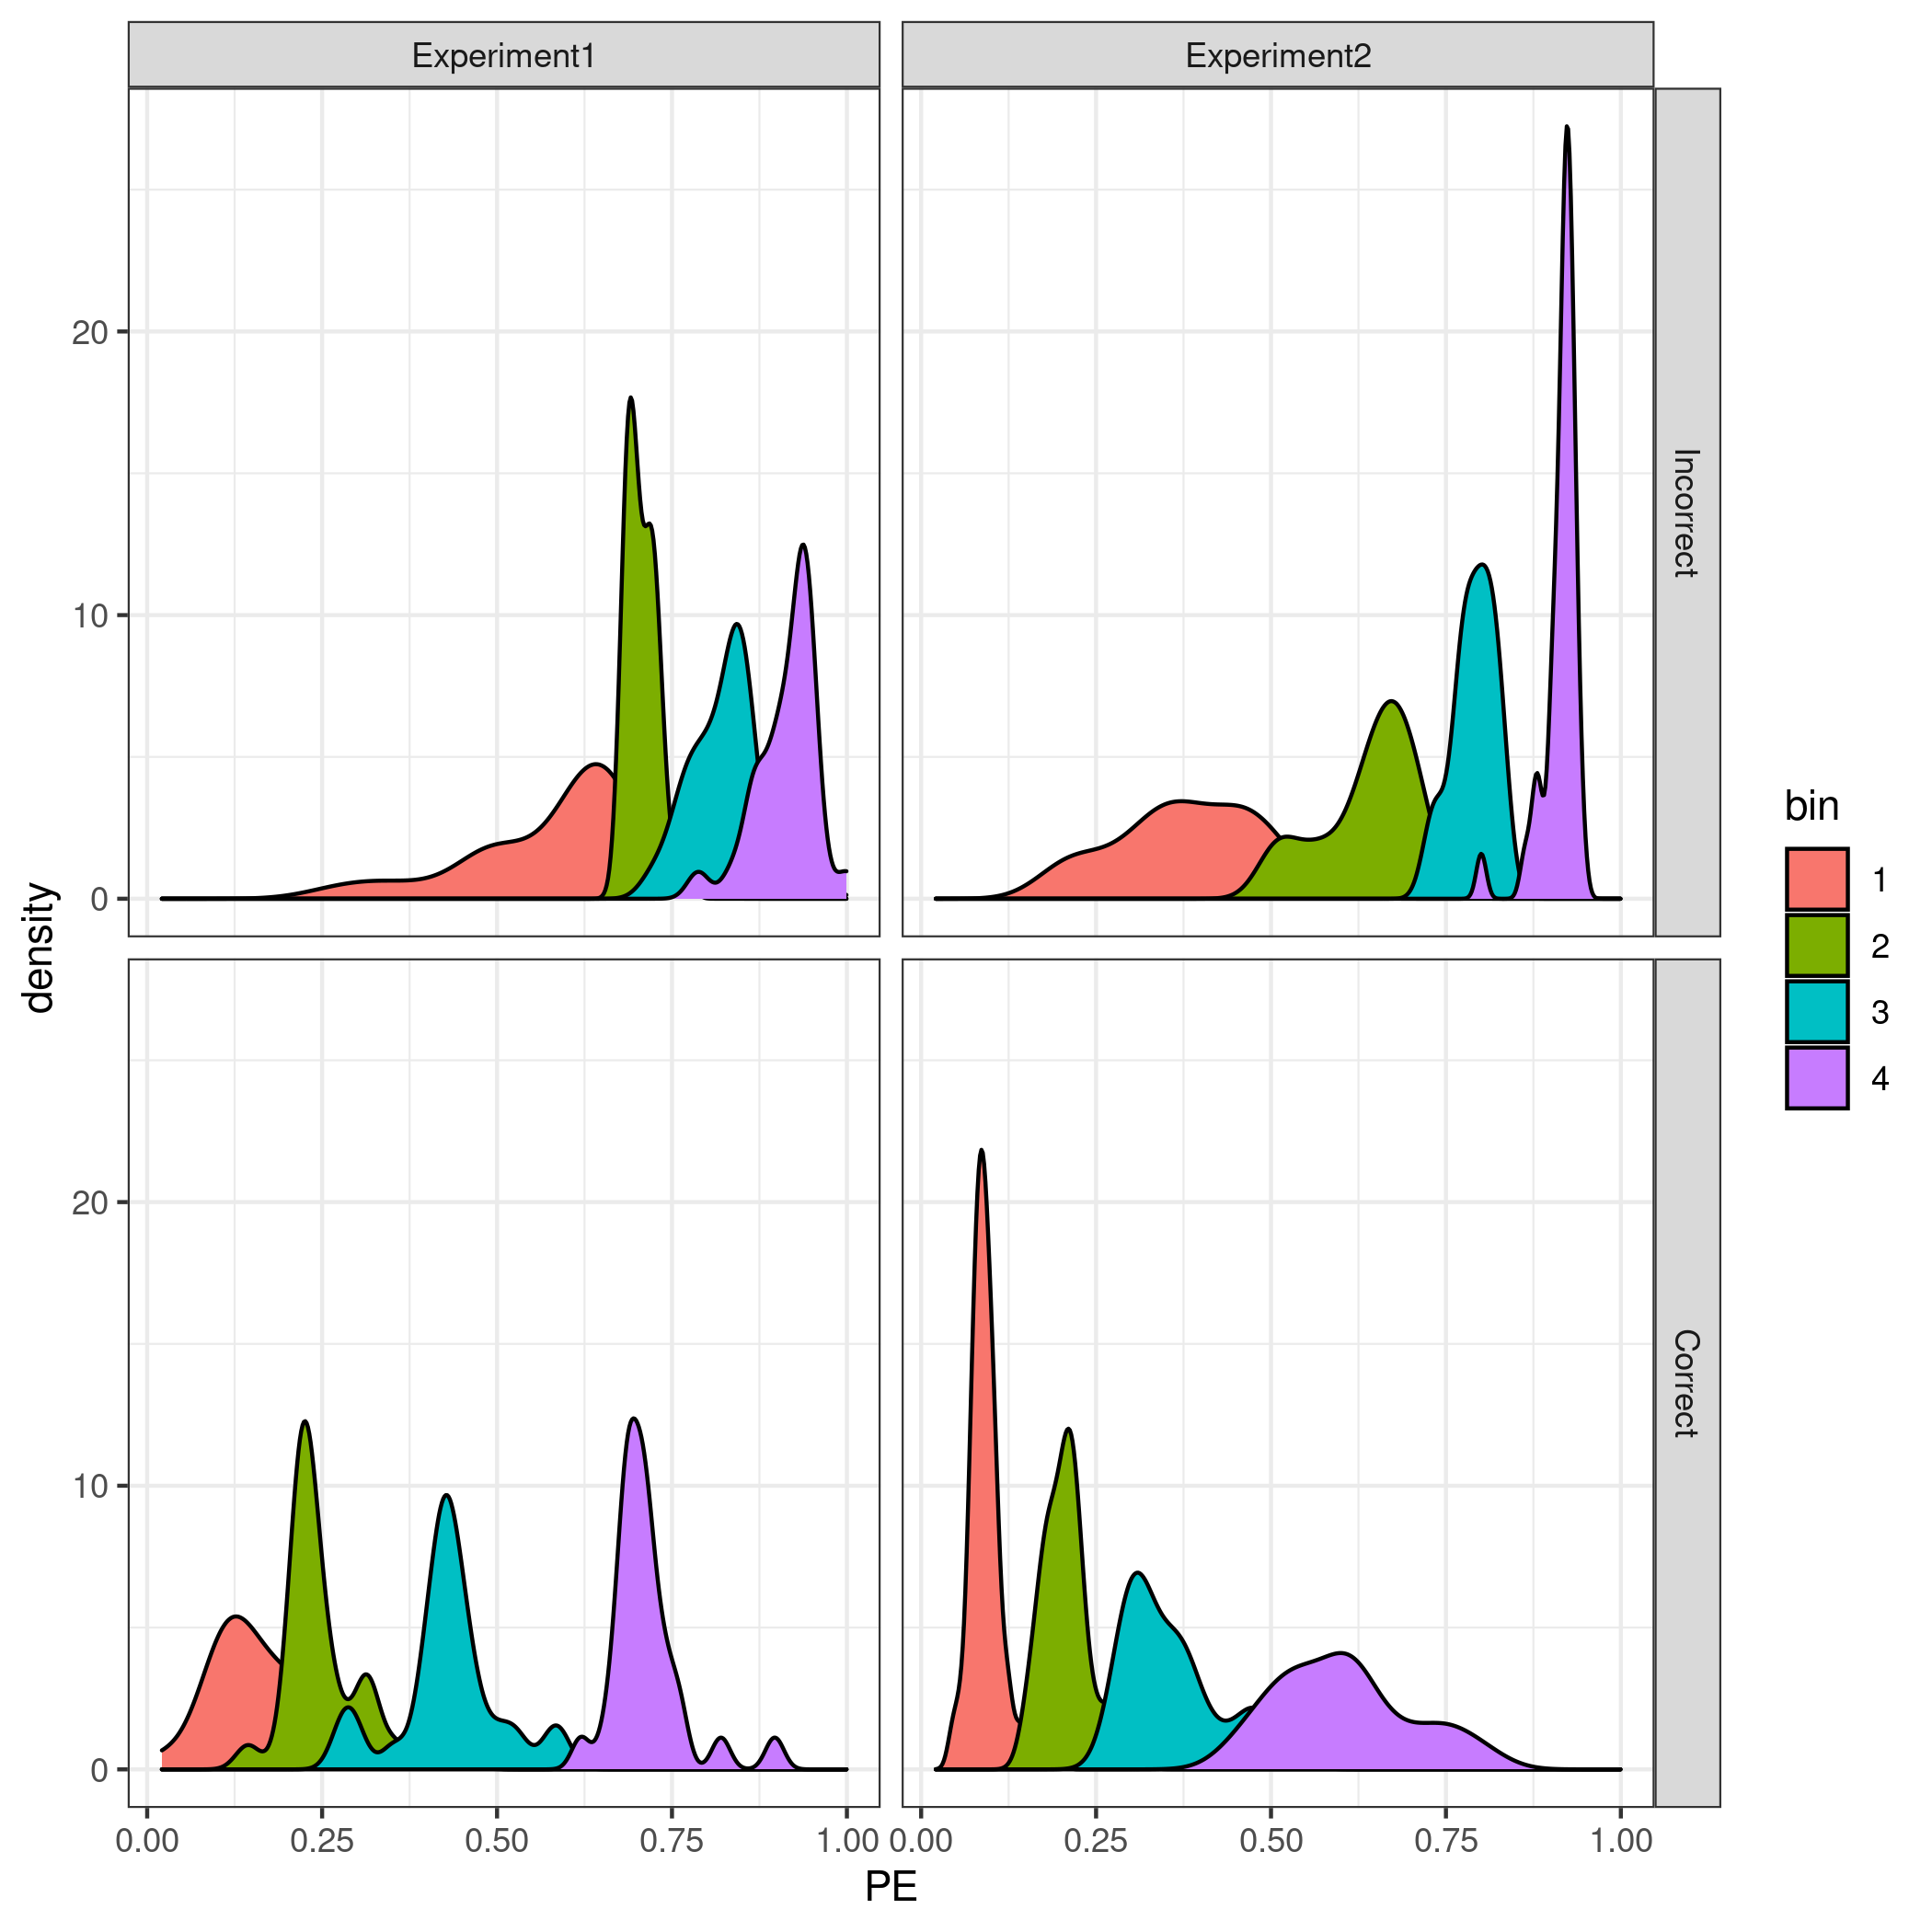
\includegraphics[width=1\textwidth]{figures/PEdistr_binned.png}}
\caption{\textbf{Distribution of binned PE.}Distribution of PE after binning it, as a function of prediction outcome and experiment. }
\label{fig:PEbin_distr}

\end{figure}

\begin{figure}[ht!]
{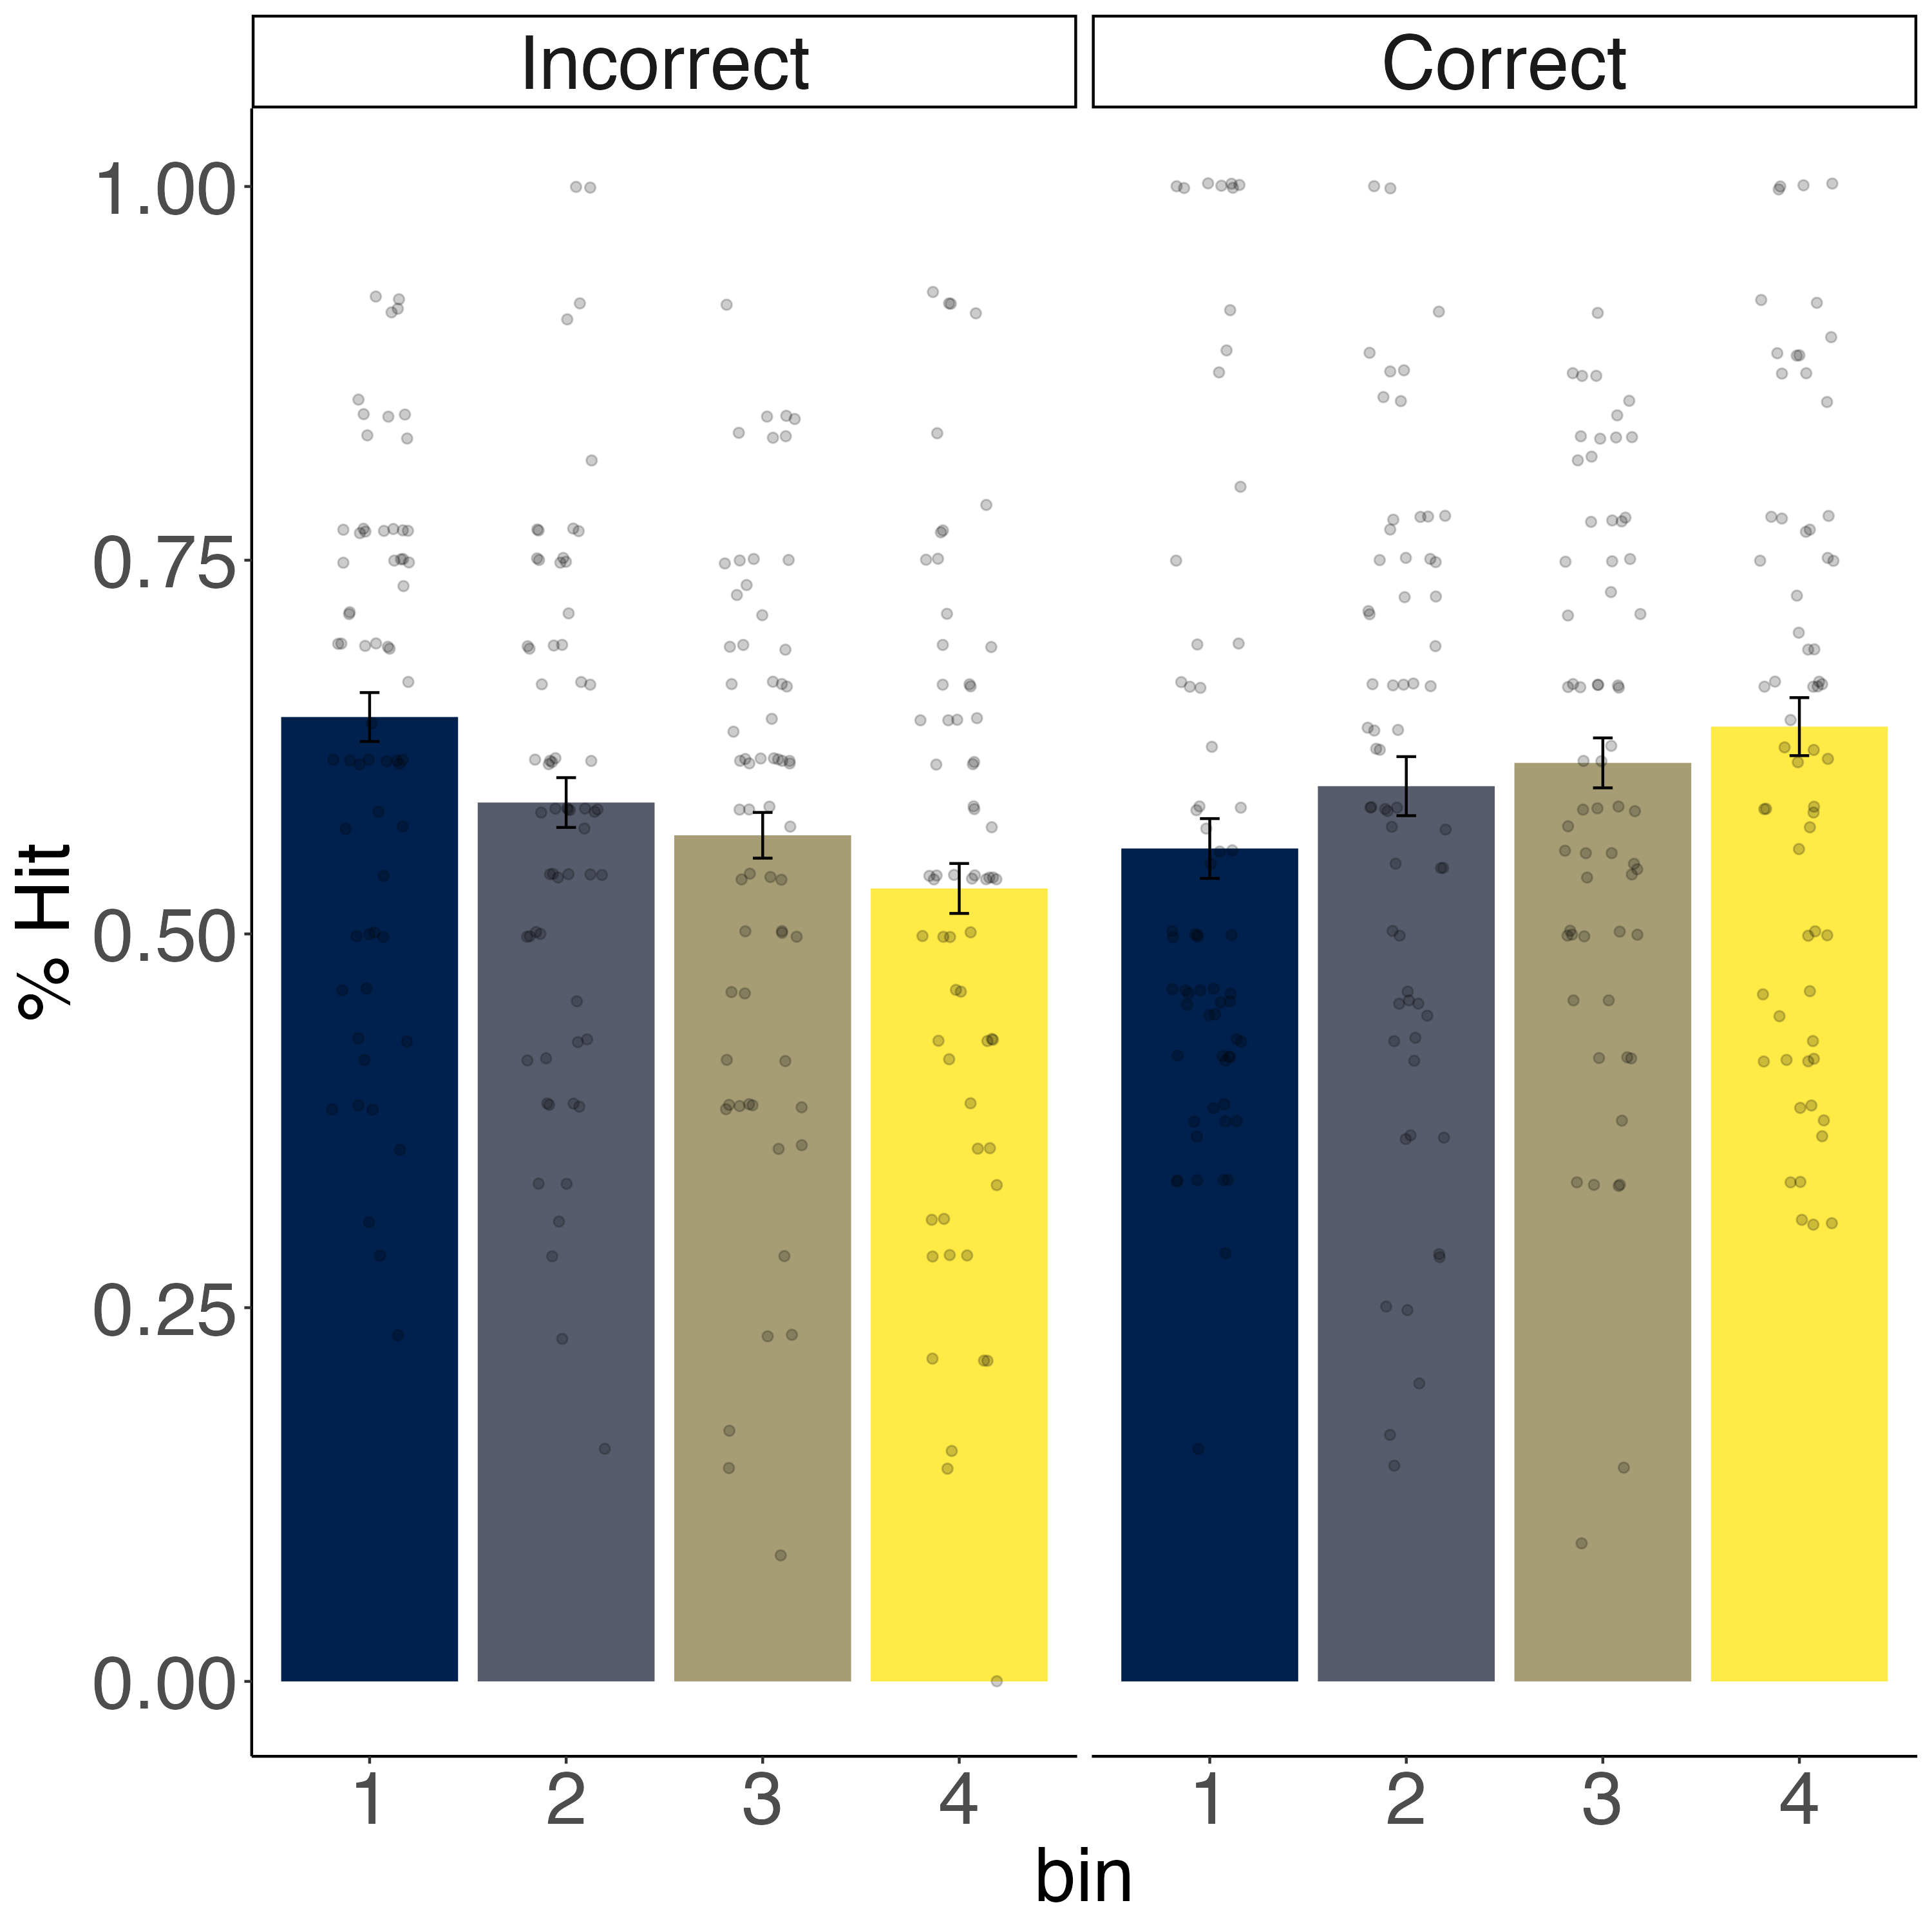
\includegraphics[width=1\textwidth]{figures/binnedPE_mem.png}}
\caption{\textbf{Hit Rate by Binned PE.} Effect of binned PE on hit rate as a function of prediction outcome. }
\label{fig:PEbin_mem}

\end{figure}

Hit rate as a function of binned PE and prediction outcome is shown in Figure \ref{fig:PEbin_mem}. 
 We then tested for the three-way interaction between binned PE, prediction outcome, and experiment, in a linear mixed-effects model, adding participants as random effects. The three-way interaction was not significant, $\chi^2_{(3)}$ = 4.23, \textit{p} = .238. In addition, the interactions between PE and experiment, and the interaction between prediction outcome and experiment were not significant ($\chi^2_{(3)}$ = 1.68, \textit{p} = .642, $\chi^2_{(3)}$ = 0.81, \textit{p} = 0.368, respectively). These results suggest that there were not significant differences in the effects of PE and in the interaction between PE and prediction outcome between the two experiments. By contrast, there was a main effect of experiment, $\chi^2_{(3)}$ = 7.70,  \textit{p} = .005,  showing that overall participants’ performance was significantly worse in Experiment 2, compared to Experiment 1. Importantly, there was also a significant interaction between PE and prediction outcome, $\chi^2_{(3)}$ = 14.09, \textit{p} = .003.\par
 To break down the interaction, the effect of PE on recognition was analyzed separately for correct and incorrect prediction outcomes. We compared each bin with the first one, to test whether increasingly higher PE significantly affected memory encoding. Results showed that for incorrect prediction outcomes, the difference between the first and the second was significant,$\beta$ = - 0.0557, $p_{corr}$ = .040, OR = 1.06. In addition, the comparisons between the third and the first, and the fourth and the first, were both significant, ($p_{corr}$ < .001). For correct prediction outcomes, the comparison between first and second quantile, and first and third quantile did not reach significance ($ps_{corr}$  >.114), whereas the comparison between the fourth and the first quantile was significant,$\beta$ = 0.081, $p_{corr}$ = .009, OR = 1.08. These results suggest that while a PE error generated by incorrect prediction impairs memory even when prior expectations are not very strong, for correct predictions a higher PE is needed in order to observe benefits for memory encoding. 

\section{Discussion}
Previous literature has provided mixed evidence on the effects of prior expectations on memory formation \citep{Bein2015, BrodGarvinShingYee2019, Greve2017, Kafkas2018}. First studies on reward PE using reinforcement learning models have also produced contrasting results \citep{Jang2019, de2018signed,Rouhani2018, Rouhani2021}. In two experiments, we analyzed the effects of PE generated by expected and unexpected events on memory encoding, by using computational models to derive trial-by-trial PE levels. We showed that prediction outcome was a strong modulator of the effects of PE on memory encoding. Namely, when unexpected events were successfully predicted, PE was beneficial to memory encoding; conversely, PE was detrimental when expected events were unsuccessfully predicted. These results reveal a computationally specific effect of PE, highlighting the crucial modulating role of prediction outcome. \par
Results showing worse memory for events eliciting PE as a result of incorrect predictions are in line with studies showing benefits of matching expectations \citep{Bein2015, BrodGarvinShingYee2019, VanKesteren2013}⁠. In fact, findings from the current study reveal that higher PE, under strong prior conditions, renders worse the memory. However, our results also show that PE can be beneficial to memory in conditions when prior expectations are low and the events are correctly predicted. These findings are in line with studies on reward PE showing better memory for better than expected outcomes \citep{de2018signed, Jang2019}, a pattern suggested to be related to dopaminergic activity promoting hippocampal plasticity and memory formation \citep{Bethus2010,Rosen2015}⁠.\par
Results from the current studies are in contrast with previous findings exploring effects of unsigned reward PE \citep{Rouhani2018, Rouhani2021}. One possible explanation for this discrepancy is the task used at encoding. While Rouhani and colleagues (\citeyear{Rouhani2018, Rouhani2021}) have used a Pavlovian task in which participants’ predictions did not affect the outcome, in the present study it was emphasized that the participants’ task was to correctly predict the object category in relation to each context. Therefore, even if episodic encoding was incidental, participants’ choice was still relevant for the task goal. \par
 Another potential explanation for the effects observed is related to the utility of the information presented. Events can be processed differently depending on whether they are useful in the future to correctly predict events in similar contexts. In fact, while positive feedback when prior expectations are weak may inform individuals that the choice is important for future similar contexts, negative feedback in contexts where prior expectations are strong may inform participants that that event is not useful for future predictions. Therefore, events that might be important to guide future behaviour may be remembered better, while those that are deviant from established expectations may be discarded as exceptions. Results are thus in line with views considering reinforcement learning as both a reward-seeking and an information-seeking system \cite{ESBromberg-Martin2011, Niv2011}⁠, emphasizing the utility of information in modifying behaviour and optimizing outcomes. \par
It is important to note that mismatched information might have been discarded as not helpful for the future because the task used in both experiments used contingencies that were established before encoding of the events and never changed during the course of the task. As a consequence, deviant information was quite expected from participants. It is possible that mismatched information would be more valued during the learning of the priors or in conditions where the environment changes instead of remaining stable, making the incongruent outcomes more unexpected. There is evidence that expected and unexpected uncertainty might have different behavioural and neurophysiological correlates \cite{Yu2005})⁠
In conclusion, the current study provides robust evidence on the effects of PE on memory encoding, highlighting the crucial modulating role of prediction outcome. 


\section{Methods}
\subsection{Participants}
In experiment 1, thirty-two young adults (20 female; mean age = 22.59 years, \textit{sd} = 3.18) were recruited through advertisements placed at the Goethe University campi in Frankfurt am Main. In exchange of participation, participants received either course credits or a monetary reimbursement of 8 €/hour. 
In experiment 2, 40 participants (19 female; mean age = 24.87, \textit{sd} = 4.64) were recruited through the Prolific platform https://www.prolific.co/). All participants had normal or corrected-to-normal vision and no history of psychological or neurological disorders. All participants gave written informed consent prior to participation. The study was approved by the ethics committee of the Goethe University Frankfurt am Main. 
\subsection{Materials}
For experiment 1, six coloured scene categories depicting real world outdoor locations taken from the ECOS database (https://sites.google.com/view/ecosdatabase/) were used as contexts. The selected scene categories were beach, mountain, road, desert, savannah, and seabed. As objects, 192 coloured images depicting real world objects were collected from an online search and were used as target objects. The images selected included the same number of objects for three different object-categories: musical instruments, fruits/vegetables, and household objects. All images were subjected to creative commons licensing and are available at https://github.com/ortiztud/premup. 
For experiment 2, the number and types of the scene categories were the same as experiment 1. By contrasts, the objects categories were reduced and only two were used: musical instruments and household objects. 
\subsection{Design and procedure}
In experiment 1, participants completed the learning, encoding, and retrieval tasks in one session, while in Experiment 2 participants completed the learning phase in a first session and the encoding and retrieval phase approximately 24 hours later. In addition, in the second session of experiment 2 participants worked on an extra reminder block of contingency learning before the encoding phase. 
In Experiment 1, stimulus presentation and recording of the responses was done using MATLAB’s Psychtoolbox (Brainard, n.d.) in a 60 Hz monitor (resolution: 1680 x 1050, full HD). 
 Experiment 2 was moved online due to the COVID-19 pandemic, and some necessary changes were implemented. Stimulus presentation and response collection were programmed in PsychoPy v2021.1.4 and hosted online in Pavlovia (https://pavlovia.org). At the beginning of each session, the experimenter met the participant in a virtual room using an online video-conferencing tool, during which the appropriateness of the testing setup was assessed with a brief set of questions about the participant’s overall well-being, about the physical room in which the task would be performed and about the computer that would be used. Experimenters ensured that all participants were sitting in a quiet room, used a laptop or a desktop computer and were encouraged to minimize distractions as much as possible during the session. At the end of the session, the experimenter met the participant again and ask them about any unforeseen event or situation that might have come up during the completion of the task. Finally, to maximize engagement, self-administered breaks were included after every 40 trials during the contingency learning and the encoding phases. 
\paragraph{Contingency learning phase.}
Participants were presented with the scene contexts on the screen and were instructed to learn which object category was more likely to belong to each of the scene contexts; they were told that some contexts were easier to learn than others, but the exact contingencies were not explicitly given. A fixation cross at the center of the screen marked the beginning of each trial and lasted for 500 ms. After that, a scene image including a rectangular white patch with a question mark was presented. They were then asked to make a prediction about the object category that they thought they would encounter in that context. Three response alternatives were given for Experiment 1 (i.e., musical instruments, fruits/vegetables, and household objects) and only two for Experiment 2 (i.e., musical instruments and household objects). Category reminders were placed at the bottom of the screen and participants could choose among them by pressing one of three arrow keys (left arrow, down arrow, right arrow) in a QWERTZ keyboard. The selected category was highlighted with a yellow frame. After 2 seconds from scene onset, the question mark within the white patch was replaced by an objects and the coloured frame changed colour to indicate correct or incorrect response. Specifically, the coloured frame around the image became red to indicate incorrect responses, and green to indicate correct responses. Object and feedback were shown on the screen for 1 second. Participants were told to use the feedback to learn the contingencies over trials. \par
The frequency to which an object category was encountered in the given scene contexts was manipulated to create different prior strengths. The prior strengths were "Flat" and "Strong" in Experiment 1, and "Flat", "Weak", and "Strong" in Experiment 2. In Experiment 1, the "Strong" prior condition consisted on three scene contexts in which one of the three object categories was frequently presented 80 \% of the trials, while the other two were equally presented 10 \% of the trials each. Conversely, the "Flat" prior condition consisted of three scene contexts in which the object categories were all three equally probable, being presented each 33 \% of trials. 
In experiment 2, the "Strong" prior condition was composed by two context scenes where one of the two object categories was presented 90 \% of the trials, while the other object category was presented on 10 \% of the trials. Two more scene contexts belonged to the "Weak" prior condition, in which the more frequently presented object category was shown on 70 \% of the trials, while the other object category appeared on 30 \% of the trials. Finally, the "Flat" prior condition included two scene contexts in which both object categories were equally likely to be presented, appearing each one on 50 \% of the trials. 
In order to achieve the desired contingencies without proportionally increasing the number of individual objects used, different objects were repeated a different number of times depending on its category and on the contexts in which they were shown. The association of each object category to each scene category was counterbalanced across participants so that across the entire sample, every object category was paired with every scene category.
\paragraph{Encoding Phase.}
The encoding Phase in Experiment 1 and 2 was similar to the learning phase, with only minor changes introduced. The explicit feedback represented by the coloured squared surrounding the object was removed in this phase, to avoid its potential effects on episodic encoding. In addition, a new set of objects was used, and each of these objects was presented only once. To equate the number of objects in each critical cell for our analysis, we selected a fixed number of objects (n=20) for each PE condition, and these were presented only once. Then, to achieve the desired contingencies for each scene category, we used filler objects from the same object categories and repeated them 7 times. Filler trials were not considered for recognition memory. \par
Similarly to the contingency learning phase, participants' task was to predict which object category followed a scene context that was presented on every trial. The contingencies between object categories and scenes were the same as the previous learning phase. 
\paragraph{Retrieval Phase.}
In the object recognition test, all the objects from encoding phase together with 192 new objects were used. 
In Experiment 1, hit rate was calculated on a sample of half of the 192 objects (96 trials), as half of the trials were selected for the immediate recognition session which is the object of the analysis of the current study, while half were selected for a delayed recognition test, which is not considered in the current study. In experiment 2, all the 192 old objects were considered for hit rate calculation. Trials started with a fixation cross for 500ms, and objects were presented in isolation at the center of the screen. Participants were required to make old/new judgements. All the responses in the retrieval phase were self-paced and not time-constrained, and the display stayed unaltered until participants made a response. After that, a new trial was then presented.
\subsection{Computational Models}
We fitted participants' data with computational models. The models considered are all different version of a standard Rescorla-Wagner model (or Q-learning) \citep{Sutton1998, Daw2011}. For each scene category, the model estimates a trial-level variable \textit{Q} for each object category included in the experiments (three in experiment 1 and two in experiment 2). These \textit{Q} values reflect the strength of participants' belief that a certain object category (for example, "Instruments") will be presented in a specific context (for example, "beach"). 
\noindent
Since we have \textit{N} object categories for each \textit{n} context, the estimates $\hat{Q}$ of the probabilities can be represented by the following \textit{c}-by-\textit{j} matrix:

\begin{equation}
\begin{bmatrix} 
\hat{Q}^{1,1}, & \hat{Q}^{1,2}, & ... \\
\hat{Q}^{2,1}, & \hat{Q}^{2,2}, & ...\\
..., &..., & \hat{Q}^{j,c} \\
\end{bmatrix}
\quad
\label{matrix}
\end{equation}

\noindent
Where $\hat{Q}^{1,1}$ represent the expected value Q for category \textit{j}=1 in context \textit{c}=1. For all the models considered in this study, the estimated values are stored in a category \textit{j} by context \textit{c} matrix as this one, and initialize as  $\hat{Q}^{j,c} = 0.33$ in experiment 1, and $\hat{Q}^{j,c} = 0.5$ in experiment 2.

\paragraph{Decreasing Learning Rate Instructive Model (dLRI)}. First, to provide a normative Bayesian solution, we used a Dirichlet-multinomial model. We applied a multinomial distribution because the categorical distribution that we used in our task is a special case of the multinomial distribution that consists of only one random sample during each trial (see Supplemental Material). The Dirichlet multinomial model can be reformulated to a delta-rule model in which the learning rate constantly decreases inversely proportional to the number of the trial. 
Thus, the delta-rule model sequentially updates the category probabilities for each context according to

\begin{equation}
\hat{Q}_{t+1}^{j,c} = \hat{Q}_{t}^{j,c}  + \dfrac{1}{t} \delta_{t},
\end{equation}


\noindent
where $\hat{Q}_{t+1}^{j,c}$ denotes the estimate of the probability of category $j$ in context ${c,j}$ at the next trial $t+1$. This estimate is based on the current estimate of the category probabilities ($\hat{Q}_{t,j}^{j, c}$) and the prediction error $\delta$, calculated as:

\begin{equation}
{\delta} = {r}_t^{j} - \hat{Q}_{t}^{j,c}
\label{eq:PE}
\end{equation}

\noindent
where the feedback ${r}_t^{j}$ represents an array of \textit{N-by-j} elements, in which each element refers to a category \textit{j}, defined as following:

\begin{equation}
r_t^j = \begin{cases}
1\ if  \ j = j_t  \\ 
0 \ otherwise
\end{cases}
\label{eq:instrPE}
\end{equation}

\noindent
 The values of the array are 1 if category \textit{j} is present on trial \textit{n}, and 0 if it is not. Therefore the model is assuming that a value estimate for an object category that appears on a trial incrementally increases as a result of a prediction error until $Q_{t}^{j,c}$ reaches its asymptote of 1. Conversely, the value estimates of categories that are not presented on trial \textit{t} decrease as a results of a negative prediction error, unless $Q_{t}^{j,c}$ for those categories has already a value of 0. 
Therefore, this model only uses instructive feedback, which indicates what is the correct choice, independently of participants' action. The learning rate $1/t =: \alpha$ indicates to which degree the prediction error influences the updated estimate of the category probabilities. Given that the learning rate in our case directly depends of the number of completed trials $t$ for a context \textit{c}, it continuously decays as a function of trials. This principle ensures that the influence of prediction errors is stronger at the beginning of the task. For more information about the formalization of the optimal Bayesian model, see Supplemental Material. 

\paragraph{Free Learning Rate Instructive Model (fLRI)}. The dLRI shows how an optimal agent should update the expected values. However, participants' behaviour may be far from optimal. %citation needed 
For this reason, the fLRI allows each participant to have its own learning rate $\alpha$. The expected values are thus updated according to the following rule: 

\begin{equation}
{Q}_{t+1}^{j,c} = {Q}_{t}^{j,c}  + {\alpha} \delta_{t},
\label{eq:fLRI}
\end{equation}

\noindent
while $\delta$ is the same as in equation \ref{eq:PE}. Also, note that this model uses the same instructive feedback as in equation \ref{eq:instrPE}.

\paragraph{Free Learning Rate Evaluative Model (fLRE)}. This model still allows participants to have a fixed learning rate $\alpha$. However, this model assumes that the feedback depends on the actions that participants take. The expected values are thus updated as follows:


\begin{equation}
{Q}_{t+1}^{j,c} = \begin{cases}
{\alpha} \delta_{t}\ if  \ a_t = j_t \  \\ 
{Q}_{t} \ otherwise
\end{cases}
\end{equation}

\noindent
where $a_t$ is the object-category selected by participants on a given trial, $\delta_{t}$ is calculated as in equation \ref{eq:PE}, and $r_t$ is 1 if the choice is the correct one, and 0 otherwise. 

\paragraph{Action Selection}. The expected \textit{Q}-values computed through the models listed above were translated into choice probabilities by implementing a softmax rule as follows: 

\begin{equation}
P_t^{j,c} = \dfrac{ exp({\beta} {Q}_t^{j,c})   }
{ \sum_{j=1}^j (exp({\beta} {Q}_t^c) },  
\end{equation}

\noindent
where $P_t^{j,c}$ represents the probability of choosing a specific object-category \textit{j} for a defined scene category \textit{c}. The inverse temperature parameter $\beta$ is another free parameter that modulates the stochasticity of the choice, with higher values meaning more deterministic actions and lower values more noise-sensitive choices. 

\paragraph{Parameter Recovery}. Before fitting the models to participants' data, a parameter recovery procedure was run for both Experiment 1 and Experiment 2, in order to check whether the fitting procedure for each model gave meaningful parameters and to find potential parameters boundaries. Fake data with randomly sampled known parameters where simulated, then the models were fit to the simulated data \citep[see][]{Wilson2019a}. The priors from which the simulation parameters were sampled are shown in table \ref{tab:priors}. In order to fit the data, we used maximum likelihood estimation (see section). Because the models are designed to reflect participants' learning, only the strong (Experiment 1) and strong and weak (Experiment 2) conditions were simulated. High correlation between simulated and fitted data indicates that the model successfully recovered the parameters that were used to generate the data. First attempts to recover the parameters allowed to set the boundaries for inverse temperature parameters. Plots of the parameter recovery are shown in figure \ref{fig:parameter_recovery}.

% The alpha parameter, the learning rate, was drawn from a uniform distribution (min=0, max =1). The beta parameter, the inverse temperature parameter, from drawn from an exponential distribution. Beta parameter was constrained at 30 after inspection of the first parameter recovery plots, as for values that are above that boundary parameter do not affect behavior much (Wilson and Collins, 2019). Stickiness parameter is drawn from normal distribution with mean 0 and sd 1.



\begin{table} 
    \centering 
    \caption{Priors for the parameters}
    \scalebox{1}{
    \begin{tabular}{l l}
     \hline
    Parameter & Priors \\
    \hline
    
 ${\alpha}$ & $\sim U(0,1)$ \\
  ${\beta}$ & $\sim exp(1)$ \\
     \hline
    \end{tabular}
}
    \label{tab:priors}
    \end{table}



\paragraph{Model Recovery}
Besides parameter recovery, another procedure to evaluate the reliability of the model is model recovery \citep{Wilson2019a}. The aim of model recovery is to determine that a model, among several ones, can successfully be indicated to be the one to have generated the data. To achieve this, data of the three different models were simulated (with randomly sampled parameters) and then fit to each of the models. The models were then compared to determine which one fitted the data best. The method used to assess the fit of the models was the Bayesian Information Criterion, \textit{BIC}, which incorporates a penalty for the number of parameters:

\begin{equation}
BIC = {-2}log \hat{LL} + k_m log{(T)},
\label{eq:BIC}
\end{equation}

\noindent
where $\hat{LL}$ is the log-likelihood value when the model is fitted with the best fitting parameter, and $K_m$ is the number of parameters in the model \textit{m}. Lower values of \textit{BIC} mean better fit. The comparison between the models for each set of generated data was repeated 100 times to generate the confusion matrices shown in figure \ref{fig:model_recovery}.



% To capture the influence of the learned category probabilities on memory consolidation, we need a model that accurately establishes contextual priors during the learning phase. As shown in Section \ref{dmn} and \ref{delta} in the Appendix (Section \ref{apppendix}), k. In Figure \ref{fig:phase_1_strong}, we provide an example of the delta rule model for categories with $\boldsymbol{\theta}=(0.8,0.1,0.1)$ and \hl{$N=24$} trials. The first row of plots shows the sampled categories across the trials. The second row of plots shows the corresponding prediction errors. For instance, at the first trial the model did expect each category with probability $\boldsymbol{\hat{\theta}}=(0,0,0)$ and observed category 1. In response to this, the model computed a prediction error $\delta_{1,1}=1$ and for the other categories $\delta_{1,2}=0$ and $\delta_{1,3}=0$. Finally, the last row of plots shows the evolution of the expected values that are updated in response to the prediction error. Figure \ref{fig:phase_1_flat} shows an example of the flat prior condition ($\boldsymbol{\theta}=0.33,0.33,0.33$). Obviously, the frequency with whichttps://www.overleaf.com/project/6040f176de7d0939c7e879efh the categories are presented is more similar compared to the strong prior condition, which is reflected in the model's learned expected value that converges to $\hat{\theta}_{n,j(c_n)} = 0.33$ for all categories.

\subsection{Parameter Estimation and Model Comparison}
The models where finally fit to participants' data in order to estimate the parameters. The parameters of best fit for each model were estimated through maximum likelihood estimation. This procedure allowed to find the parameters $\theta$ that maximize the likelihood of the data given the parameters $p(d_{1:t} | \theta, m )$. 
The probability of the whole dataset \textit{d} is calculated as the product of the choice probabilities $p(c_t | d_{1:t-1}, \theta, m)$. As the product of the choice probabilities is often a very small number, it is common practice to use the log-likelihood instead, which is the sum of the log of the choice probabilities \cite{Daw2011, Wilson2019a}:

\begin{equation}
LL = \sum_{t=1}^{n} \log{p(c_t | d_{1:t-1} , \theta, m)}
\end{equation}

\noindent
where $p(c_t | d_{1:t-1}, \theta, m)$ is the probability of each single choice given the parameter $\theta$, the model \textit{m}, and all the data up to that point. \par
The search over the full set of free parameters was optimized through the package \textit{optim} in R, which was fed with the negative log likelihood and a set of starting points randomly selected from the priors shown in Table \ref{tab:priors}. The $\alpha$ parameter was constraint between 0 and 1, while the $\beta$ parameter between 0 a and 10, as parameter recovery shown that for values that exceeded 10 the model could not distinguish between different beta parameters. Because the optimizer may find a local rather than a global, we run the search for the best parameters five times, starting from different points, and then used the best winning parameters among the five iterations, i.e. the parameters that minimized the log-likelihood. 
After estimating the parameters, a \textit{BIC} value(see equation \ref{eq:BIC}) was computed for each model and for each participant using the parameters of best fit. \par
To compare the fit of the models, we calculated the average \textit{BIC} across all subjects for each model, then counted the number of participants for which each model was the best fit. In addition, we used the model evidence of the best model within each participant: Following \cite{raftery1995bayesian} and \cite{gluth2017attraction}, model evidence was defined as "weak", "positive", "strong", or "very strong" depending on the \textit{BIC} difference between the best and the second best model for each participant. Precisely, evidence was "weak" when the \textit{BIC} difference between best and second best model was below 2, "positive" when it was between 2 and 6, "strong" when it was between 6 and 10, and "very strong" when it was above 10. 

\subsection{Statistical Analysis}
In order to test the statistical significance of the effects of interest, we used linear mixed-effect models and generalized linear mixed-effect models, implemented in R through the package \textit{lmr4}. Because our main outcome variable (memory) is binary, we used the logit link function in the binomial family to fit the models to accuracy data. Participants were modelled as random intercepts, while the explanatory variables and their interactions were modelled as both fixed and random effects. The resulting generalized linear-mixed effect model can be formalized as the following:

\begin{equation}
p(Hit) =   \dfrac{1}{1+exp - (\beta_0 +\beta_{1_j} PE +\beta_{2_j} PO + \beta_{3_j} PE \cdot PO + u_{i,j} )}
\end{equation}

\noindent
where $\beta_0$ represents the fixed intercept (i.e. the average $p(Hit)$), $\beta_{1_j}$PE the fixed effect of PE,  $\beta_{2_j}$PO the fixed effect of prediction outcome, and $\beta_{3_j} PE \cdot PO$ the fixed interaction between PE and prediction outcome. Finally, $u_{i,j}$ represents the participant unique random effects, for the intercept, main effects, and their interactions.
The variance-covariance matrix for the random effects was set as unstructured. Therefore, we used the maximal random effect structure justified by the design \citep{barr2013random}. The test of the significance of the parameters was obtained through Wald chi-square test. Effect sizes were reported as odds ratios exp($\beta$), where:

\begin{equation}
Odds =   \dfrac{p(Hit=1)}{1-p(hit=1)}
\end{equation}

\noindent
In the analysis of the effect of binned PE, we used a linear mixed-effect model, with hit rate as response variable:

\begin{equation}
Hit Rate =   \dfrac{hits}{hits+missed}.
\end{equation}

\noindent
Binned PE was treated as a categorical variable with four levels. Testing for significance of planned contrasts was corrected for multiple comparison by using Bonferroni correction:

\begin{equation}
p_{corr} =   p \cdot k, 
\end{equation}

\noindent
where\textit{p} is the \textit{p} value of the comparison and \textit{k} is the overall number of comparisons considered in a model. 




\bibliographystyle{apalike}
\bibliography{library} 

%%%%%%%%%% Merge with supplemental materials %%%%%%%%%%
\pagebreak
%\widetext
\begin{center}
\textbf{\large Supplemental Materials}
\end{center}
%%%%%%%%%% Merge with supplemental materials %%%%%%%%%%
%%%%%%%%%% Prefix a "S" to all equations, figures, tables and reset the counter %%%%%%%%%%
\setcounter{equation}{0}
\setcounter{figure}{0}
\setcounter{table}{0}
\setcounter{page}{1}
\makeatletter
\renewcommand{\theequation}{S\arabic{equation}}
\renewcommand{\thefigure}{S\arabic{figure}}
\renewcommand{\bibnumfmt}[1]{[S#1]}
\renewcommand{\citenumfont}[1]{S#1}

%%%%%%%%%% Prefix a "S" to all equations, figures, tables and reset the counter %%%%%%%%%%
\section{Supplemental Material}
\subsection*{Dirichlet-multinomial model}
We will start with an application of the Dirichlet-multinomial model to all $N$ trials of the learning phase. We apply the Multinomial distribution because the Categorical distribution that we use in our task is a special case of the Multinomial distribution that consists of only one random sample during each trial (see ''Multinomial distribution'' in the Appendix). The Dirichlet distribution is the conjugate distribution of the Multinomial distribution and can therefore be utilized as a prior. 

\paragraph{Likelihood}
After the observation of $N$ pictures during the learning phase, the likelihood of the data $\boldsymbol{\mathcal{D}}=\{x_1,...x_N\}$, where $x_i \in \{1,...,K\},$ can be denoted as

\begin{equation}
p(\boldsymbol{\mathcal{D}}|\boldsymbol{\theta})= \prod^K_{k=1}\theta^{N_k}_k 
\end{equation}

where $N_k = \sum_{i=1}^{N}\mathbb{I}(y_i=k)$. Intuitively, $\boldsymbol{\mathcal{D}}$ denotes the observed data with each $x_i$ indicating how often each category was shown during the learning phase. Please note the similarity to the Categorical distribution that was introduced in ''Formal description of the task''. The major difference is that we now consider all trials of the learning phase.

\paragraph{Prior}
The prior is the Dirichlet distribution
\begin{equation}
\begin{aligned}
p(\boldsymbol{\theta}) & = \mathrm{Dir}(\boldsymbol{\theta}|\boldsymbol{\alpha})\\
&\triangleq \dfrac{1}{B(\boldsymbol{\alpha})} \prod^K_{k=1}\theta_k^{\alpha_{k-1}}\mathbb{I}(\mathrm{x}\in S_K).	
\end{aligned}
\end{equation}
In our case, the Dirichlet distribution is used to model our prior expectations (i.e., at the beginning of the learning phase) about the category probabilities, which is often referred to as pseudo-counts. The parameter that reflects our prior is denoted by $\boldsymbol{\alpha}$. I think it is fair to assume that participants start the task with a flat prior that reflects that all categories are equally likely, which corresponds to $\boldsymbol{\alpha} = (1,1,...,1)$. These values thus indicate the assumption that each category has been pseudo-counted once. For a few more details about the Dirichlet distribution see ''Dirichlet distribution'' in the Appendix and \cite{Murphy2012}.

\paragraph{Posterior}
The posterior is a Dirichlet distribution that results from multiplying the likelihood by the prior

\begin{equation}
\begin{aligned}
p(\boldsymbol{\theta}|\boldsymbol{\mathcal{D}})
&\propto p(\boldsymbol{\mathcal{D}}|\boldsymbol{\theta})p(\boldsymbol{\theta})\\
&\propto \prod^K_{k=1} \theta^{N_k}_k \theta_k^{a_{k}-1} \\
&= \prod^K_{k=1} \theta^{\alpha_k+N_{k}-1}_k \\ 
&= \mathrm{Dir}(\boldsymbol{\theta}|\alpha_1 + N_1,...,\alpha_K + N_K).
\end{aligned}
\end{equation}
The only operation that is required here is thus the addition of the observed data to the prior. This affords a simple application of the model without the need for complex computations.

\paragraph{Maximum a posteriori and maximum likelihood estimate}
In order to obtain an estimate of the category probabilities, we can compute the expected value of the posterior to obtain the maximum a posteriori (MAP) estimate:
\begin{equation}
\hat{\theta}_k = \dfrac{N_k+\alpha_k-1}{N+\alpha_0-K}.
\end{equation}
Under the assumption that $\boldsymbol{\alpha} = (1,1,...,1)$, the MAP estimate is equal to the maximum likelihood (ML) estimate that is based on the empirically observed frequency of the categories:
\begin{equation}
\hat{\theta}_k = \dfrac{N_k}{N}.
\label{eq:dmm}
\end{equation}
We already noted that in this simple version of the task, we are only required to count our observed categories. Now we additionally know that the category probabilities can simply be obtained by computing the empirical fraction of the number of times each category was presented. This affords a straightforward reformulation of our Dirichlet-multinomial model into an iterative prediction error correcting scheme.


\subsection{Delta-rule formulation}\label{delta}

We now show how eq. \ref{eq:dmm} can be translated into the delta rule. Let $\hat{\theta}_{n,j}$ denote the estimate of the $j$th category probability at trial $n$, then the estimate of the $j$th category at trial $n+1$, denoted by $\hat{\theta}_{n+1,j}$, can be computed according to 


\begin{equation}
\begin{aligned}
\hat{\theta}_{n+1,j} &= \dfrac{n_{j}}{n} \\ 
&= \dfrac{1}{n}n_{j} \\ 
&= \dfrac{1}{n}\sum_{i=1}^{n}x_{i,j} \\
&= \dfrac{1}{n}\Big(x_{n,j} + \sum_{i=1}^{n-1}x_{i,j}  \Big) \\
&= \dfrac{1}{n}\Big(x_{n,j} + (n-1)\hat{\theta}_{n,k} \Big) \\
&= \dfrac{1}{n}\big(x_{n,j}+n\hat{\theta}_{n,j}-\hat{\theta}_{n,j}\big) \\
&= \hat{\theta}_{n,j} + \dfrac{1}{n}(x_{n,j} - \hat{\theta}_{n,j}),
\end{aligned}
\label{eq:model}
\end{equation}
where $(x_{n,j}-\hat{\theta}_{n,j}) =: \delta_{n,k}$ corresponds to the prediction error and the learning rate is defined as $\dfrac{1}{n}=:\alpha_{n,j}$ \citep{Sutton1998}.

\subsection*{Dirichlet distribution}

\paragraph*{Probability simplex}

\begin{equation}
S_K = \{\mathbf{x} : 0\le x_k \le 1, \sum^K_{k=1}x_k=1\}
\end{equation}

\paragraph*{Probability density function}

\begin{equation}
\mathrm{Dir}(\boldsymbol{\mathrm{x}}|\boldsymbol{\alpha}) \triangleq \dfrac{1}{B(\mathbf{\boldsymbol\alpha})} \prod^K_{k=1}x_k^{\alpha_{k-1}}\mathbb{I}(\boldsymbol{\mathrm{x}}\in S_K)	
\end{equation}

where

\begin{equation}
B(\boldsymbol{\alpha}) \triangleq \dfrac{\prod_{k=1}^K \Gamma(\alpha_k)}{\Gamma(\alpha_0)} 	
\end{equation}

and where


\begin{equation}
\alpha_0 \triangleq \sum_{k=1}^K\alpha_k.
\end{equation}


\subsection*{Multinomial distribution}

Let $\boldsymbol{\mathrm{x}}=(x_1...x_K)$ be a random vector, where $x_j$ denotes the number of times picture $j$ in the current context occurs.

\paragraph*{Probability mass function}

\begin{equation}
\mathrm{Mu}(\boldsymbol{\mathrm{x}}|n,\boldsymbol{\theta}) \triangleq \binom{n}{x_1...x_k} \prod^{K}_{j=1}\theta_j^{x_j}
\end{equation}
where

\begin{equation}
 \binom{n}{x_1...x_k}\triangleq\dfrac{n!}{x_1!x_2!...x_3!}.
\end{equation}
In case of $n=1$:

\begin{equation}
\mathrm{Mu}(\boldsymbol{\mathrm{x}}|1,\mathbf{\theta})= \mathrm{Cat}(x|\boldsymbol{\theta})\triangleq \prod^K_{j=1}\theta^{\bold{I}(x_j=1)}
\end{equation}

%\bibliographystyle{apalike}
%\bibliography{library} 

%\bibliographySM{library}

\begin{figure}[ht!]
\centerline
{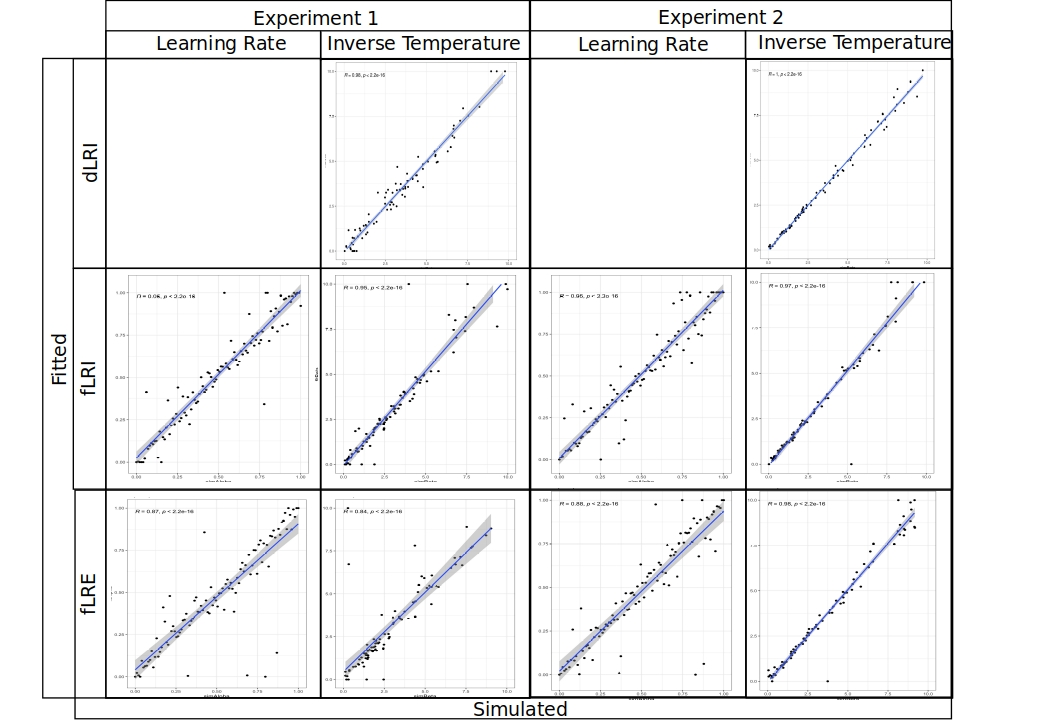
\includegraphics[width=1.5\textwidth]{figures/ParameterRecoveryAll.jpg}}
\caption{\textbf{Parameter Recovery.} Parameter Recovery for the two experiments and for the three models.}
\label{fig:parameter_recovery}
\end{figure}

\begin{figure}[ht!]
\centerline
{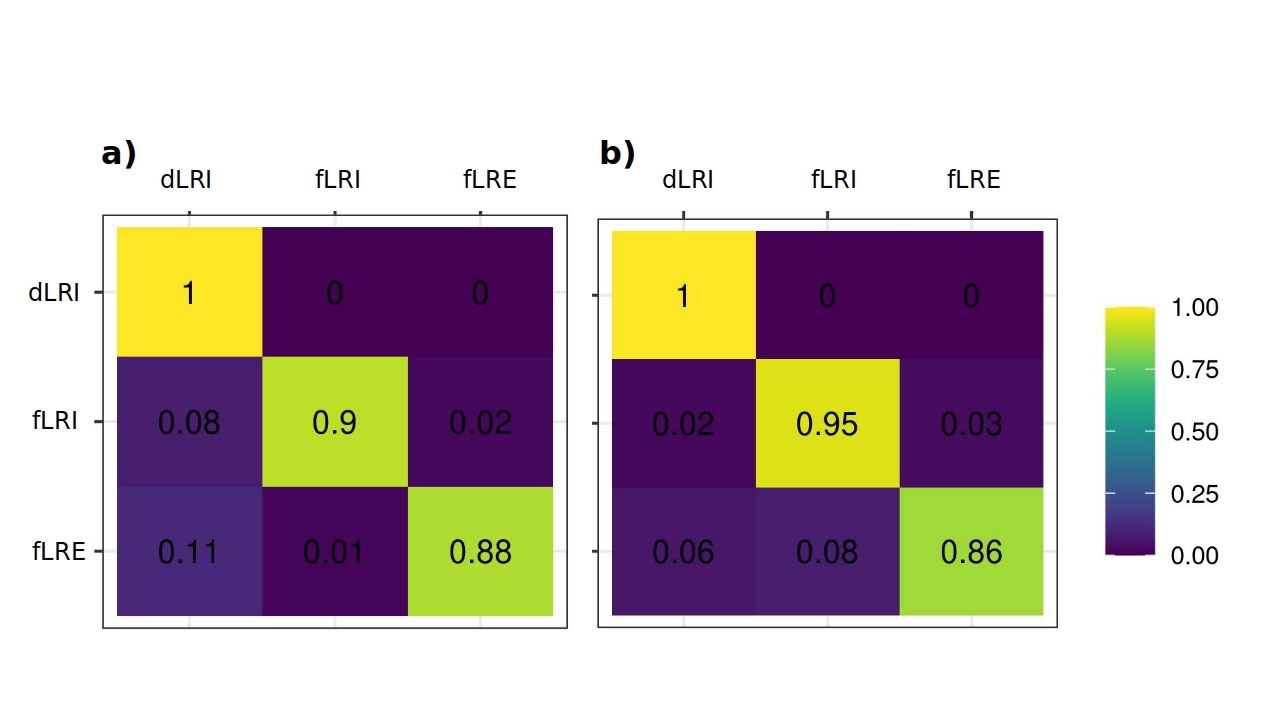
\includegraphics[width=1\textwidth]{figures/ModelRecovery.jpg}}
\caption{\textbf{Model Recovery.} Confusion Matrices showing model recovery for a) experiment 1 and b) experiment 2. The numbers show the probability of data generate by model X to be best fit by model Y.}
\label{fig:model_recovery}
\end{figure}

\end{document}